\label{results}

\section{Summary}

We present our results in three parts. 

In \autoref{validation}, we use \texttt{MorphCT} to test the performance of \texttt{pySCF} at the level of the chromophore.
Two experiments are reported. In the first, we calculate the frontier molecular orbital
energies for fused ring oligomers of increasing length. We compare the results of our experiment to the
results of the same experiment done with more rigorous DFT methods. In the second, we test the 
performance of the \texttt{pySCF} dimer calculations outlined in \autoref{methods}. 
We take two simple chromophores, two thiophene rings, in $5680$ orientations and calculate the
electronic coupling between them. We do so to test if our dimer calculation correlates sensibly to the angle
and distance between chromophores. These experiments are broadly meant to confirm that we have integrated
\texttt{pySCF} into \texttt{MorphCT} properly, and that the quantities produced comport with the physics of these systems.
We then deploy \texttt{MorphCT} on three benchmark \glsxtrshort{p3ht} morphologies to obtain charge mobility
and compare the results to previously reported values for these morphologies. This section is meant to
validate the current implementation of \texttt{MorphCT} against a previous implementation. 

In \autoref{sensitivity}, we test the sensitivity of our \texttt{MorphCT}
calculated mobilities to $d_{cut}$, chromophore
reorganization energy, \glsxtrshort{kmc} temperature, and choice of charge carrier lifetimes for \glsxtrshort{msd} analysis. Using a
benchmark \glsxtrshort{p3ht} morphology, holding all other parameters constant and sweeping across relevant scales
provides context for how to treat these parameters in future investigations. 

In \autoref{itic}, we deploy our data pipeline on \gls{itic} to obtain charge mobility. 

\section{Validation}

\label{validation}

\subsection{Quantum Chemical Calculation Validation}

As outlined in \autoref{qccmethods}, \glsxtrshort{qcc} is used in two distinct way in our workflow. 
First it is used to estimate free energy
difference between individual chromophores as the difference in their \glsxtrshort{homo} (or \glsxtrshort{lumo}) energy levels.
Secondly, it is used to estimate the electronic overlap ($T_{ij}$) with the dimer splitting method which involves
calculating the \glsxtrshort{homo} (or \glsxtrshort{lumo}) of the dimer formed by the two chromophores. We present the results from two
experiments meant to evaluate \texttt{pySCF}'s suitability for performing these duties:
(1) we compare frontier molecular energies of single chromophores given by \texttt{pySCF} to those
given by more rigorous \textit{ab initio} DFT and (2) we evaluate performance \texttt{pySCF}'s dimer calculation.

\subsubsection{Experiment 1 Methods}

At the level of a single chromophore, we calculate the \glsxtrshort{homo}-\glsxtrshort{lumo} gap for fused-ring
oligomers of increasing length. 
The difference between the \glsxtrshort{homo} and \glsxtrshort{lumo} energy levels, the \glsxtrshort{homo}-\glsxtrshort{lumo} gap, is an approximation of the amount
of energy necessary to promote an electron to a higher energy level.  
Fused-ring geometries are of particular interest for accepter
molecules, as discussed for \glsxtrshort{frea}s in the introduction. 
The fused thiophenes in this experiment represent a generic \glsxtrshort{frea} core, whose frontier molecular oribitals are
the landing cites for a charge propagating through an acceptor material. 

To recreate these experiments, using \texttt{mBuild} \cite{Klein2016}, oligomers composed of 4-8 planar fused thiophene rings
were initialized and saved to a \texttt{gsd} file. The \texttt{gsd} files were fed into \texttt{MorphCT} which uses \texttt{pySCF} to quantify the
frontier orbital energy levels \autoref{qccmethods}.

\subsubsection{Experiment 1 Results}

\begin{figure}
  \center
  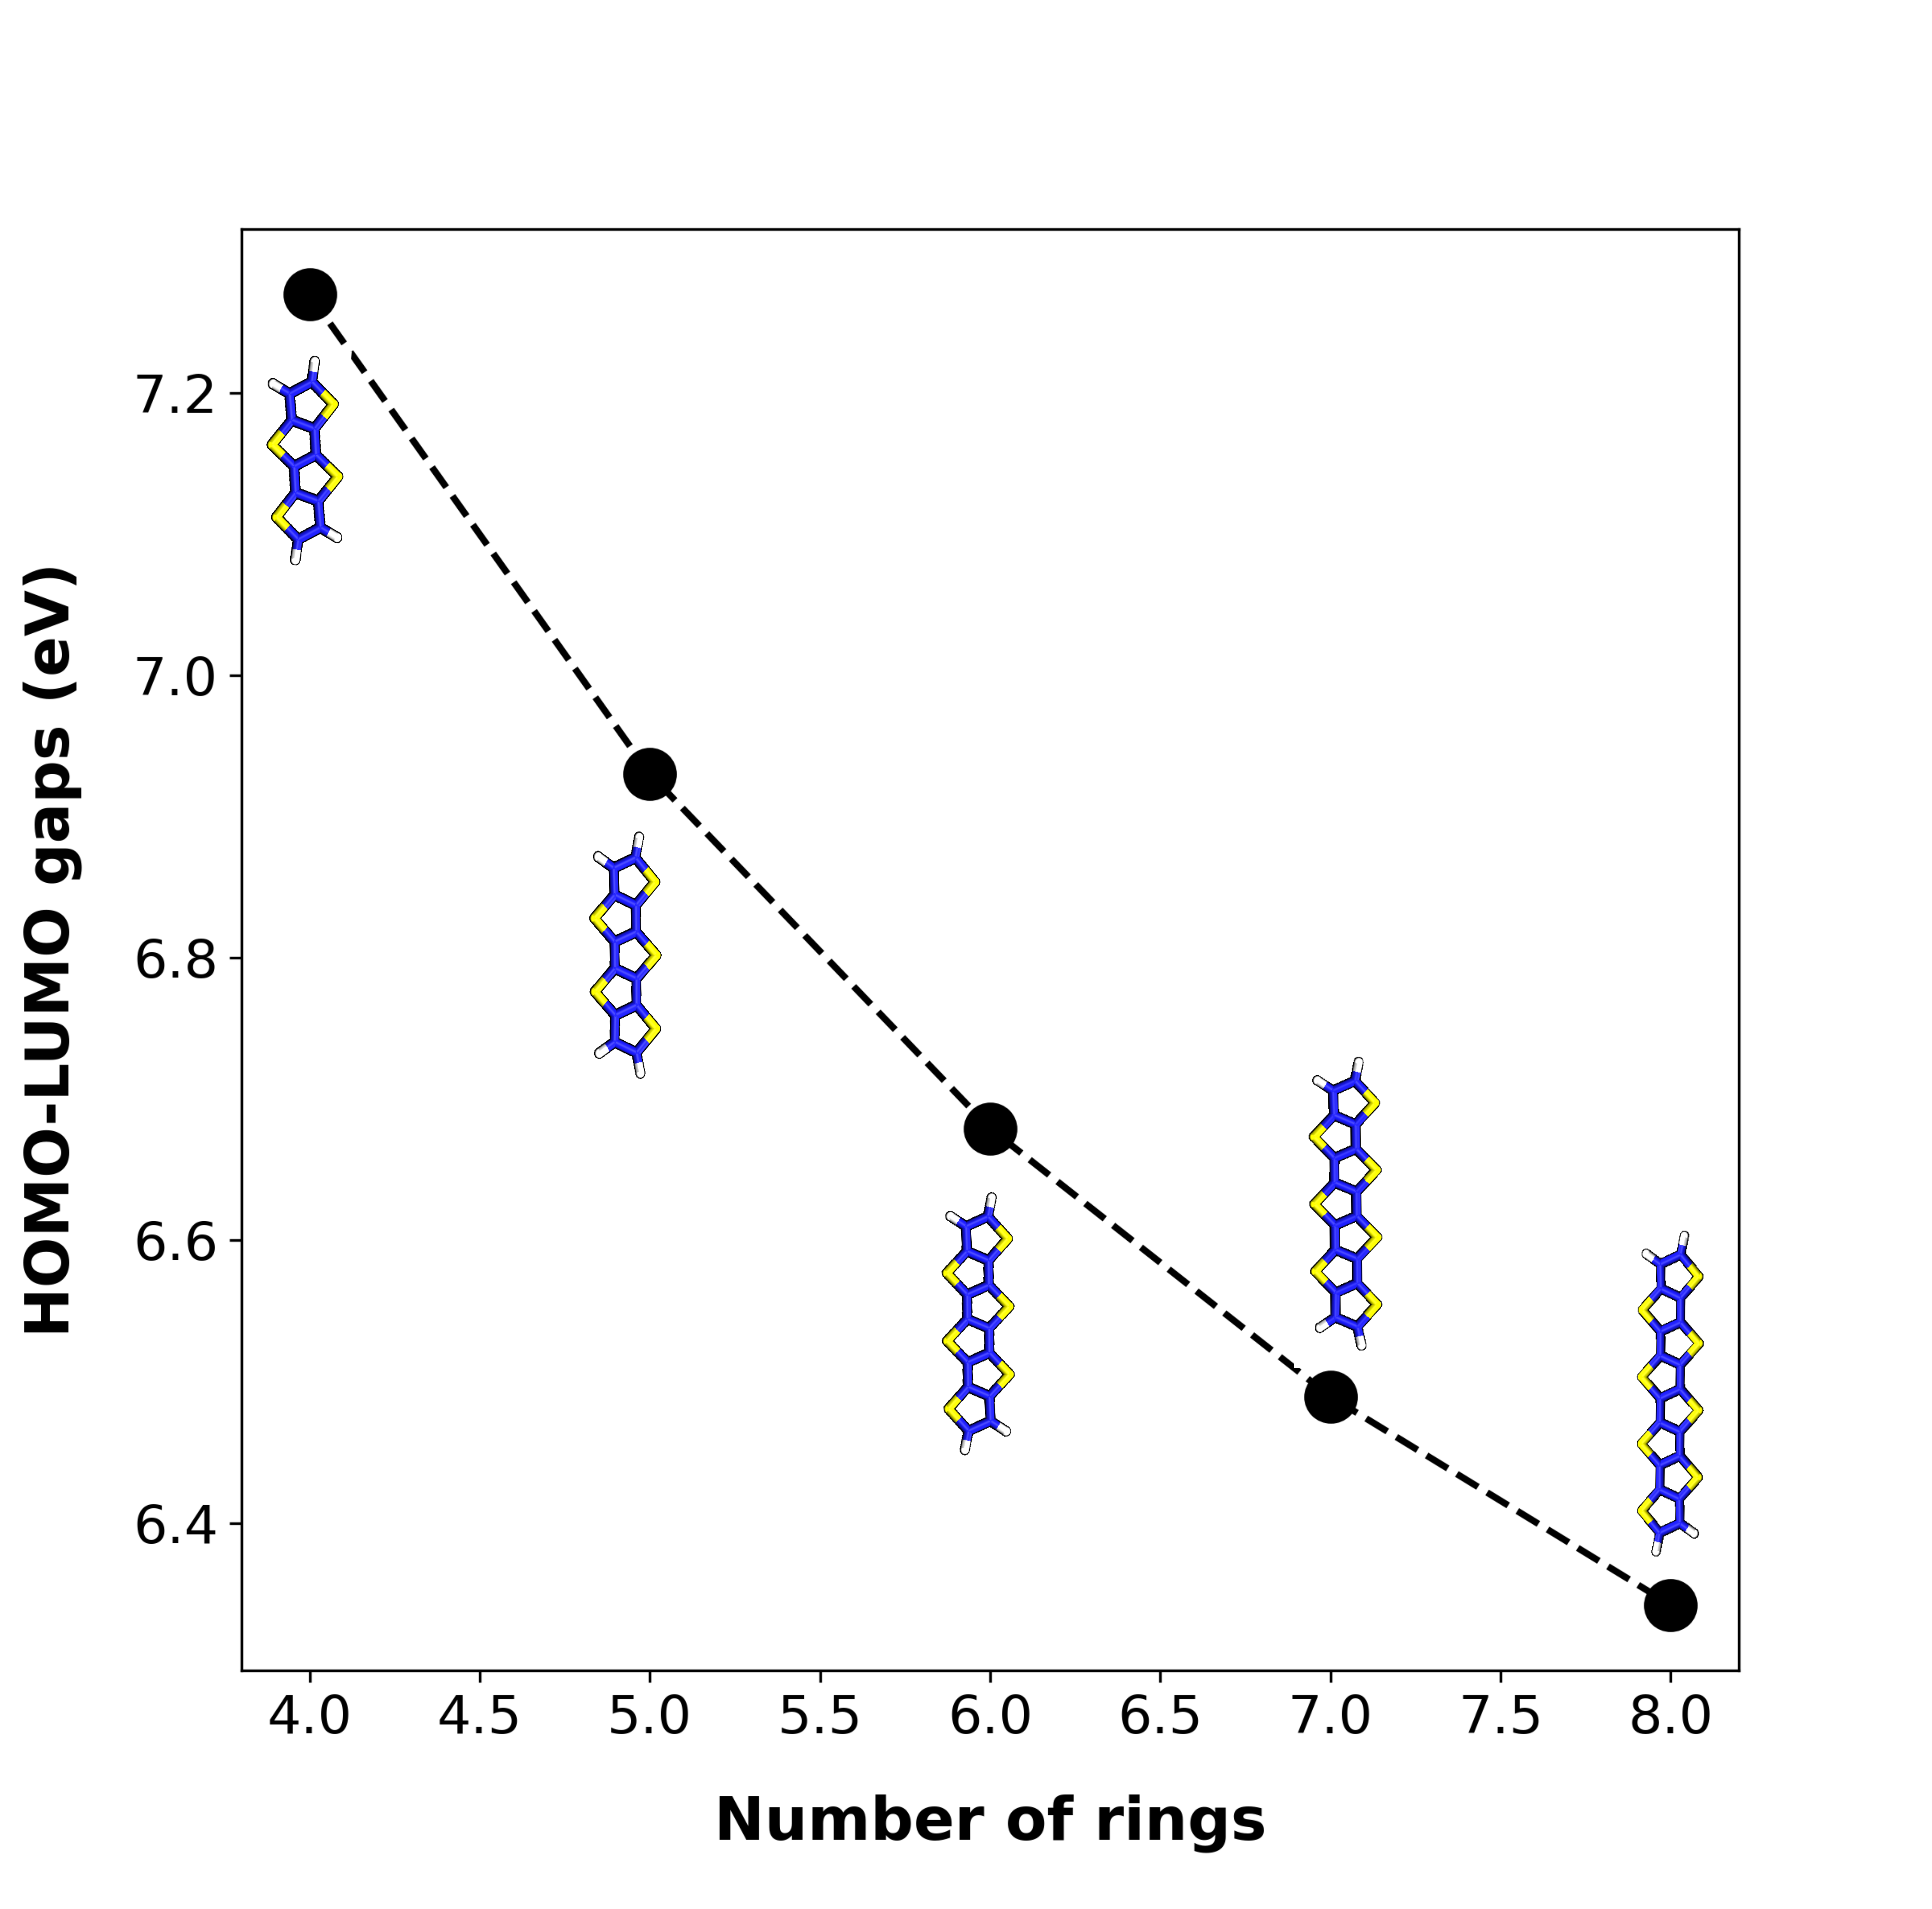
\includegraphics[width = .6\textwidth]{figures/fused-ring-figure.png}
  \caption{\glsxtrshort{homo}-\glsxtrshort{lumo} gaps obtained using \texttt{MorphCT} for fused-ring molecules of oligmer length $4-8$.}
  \label{fig:fused}
\end{figure}

Our values for the \glsxtrshort{homo}-\glsxtrshort{lumo} gap are plotted by oligomer length in \autoref{fig:fused}. 
Our \glsxtrshort{homo}-\glsxtrshort{lumo} gap ranges between $7.27eV$ and $6.34eV$. Consistent with our findings using a larger data set
in \autoref{itic}, the wall time for these individual calculations take place on the order of seconds. 

Furthermore, it is known that there is a near linear
relationship between \glsxtrshort{homo}-\glsxtrshort{lumo} gap and oligomer length. We find that our use of \texttt{pySCF} (MINDO/3) replicates
this trend and this is clear from \autoref{fig:fused}.

Our absolute values are in the range expected for INDO methods, which are known to overestimate DFT values by a factor of 2-3 \cite{Gorelsky2001}.
Our \gls{homo}-\gls{lumo} gap values compare well to those found using
\textit{ab initio} DFT (between $5.26eV$ and $4.92eV$). 

\subsubsection{Experiment 2 Methods}

At the level of the chromophore pair, we explore the effect of angle and distance on the electronic orbital
overlap, $T_{ij}$, between two non-bonded thiophene rings.
Two thiophene rings are positioned in electronic proximity using \texttt{mBuild} and saved to \texttt{gsd}. 

A reference thiophene was placed at the origin in the xy-plane
with the y-axis running through the sulfur atom as shown in \autoref{TIplots}(a). For the second thiophene,
two sets of 12 rotations about the x-axis and z-axis (with $- \frac{\pi}{2} < \theta< \frac{\pi}{2}$)
and two sets of 12 translations between $0nm$ and $0.5nm$ along the x-axis and z-axis were defined.
The Cartesian product of these sets define a space of $12^{4}= 20736$ orientations for second thiophene. 

Orientations resulting in atoms that were less
than $0.3nm$ were removed from the data set as distances shorter than this are considered
unphysical. The remaining $5680$ atomic arrangements were saved to a \texttt{gsd} and the $T_{ij}$ was quantified for
each with \texttt{MorphCT}. 

\subsubsection{Experiment 2 Results}

The data resulting from this experiment, $5680$ orientations of electronically 
interacting non-bonded thiophenes and the
corresponding $T_{ij}$ between them, provide evidence that \texttt{MorphCT} is rationally capturing the orbital
overlap between chromophores. 
The $T_{ij}$ resulting from these $5680$ orientations are shown in \autoref{TIplots}. 
The figure shows that, as expected, a decrease in 
center-to-center distance results in more orbital overlap and thus an increase in $T_{ij}$. 
Also observable in the figure is that
a negative rotation about the x-axis orients the sulfur downward, resulting in a smaller sulfur-to-sulfur distance 
and a greater $T_{ij}$. 

\begin{figure}
\centering
\begin{subfigure}{.9\textwidth}
    \centering
    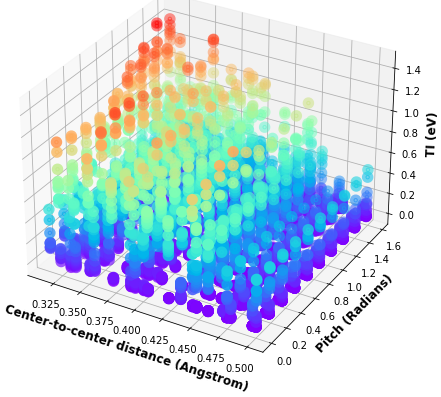
\includegraphics[width=\textwidth]{figures/transfer_integral_plot.png}
    \caption{Individual dots correspond to $5680$ 
    distinct combinations of rotations and translations of the upper
    thiophene.
    Dots are colored based on the $T_{ij}$ between thiophenes for the given x-axis rotation,
    z-axis rotation, and center to
    center distance from the reference thiophene.}
\end{subfigure}
\\
\begin{subfigure}{.9\textwidth}
    \centering
    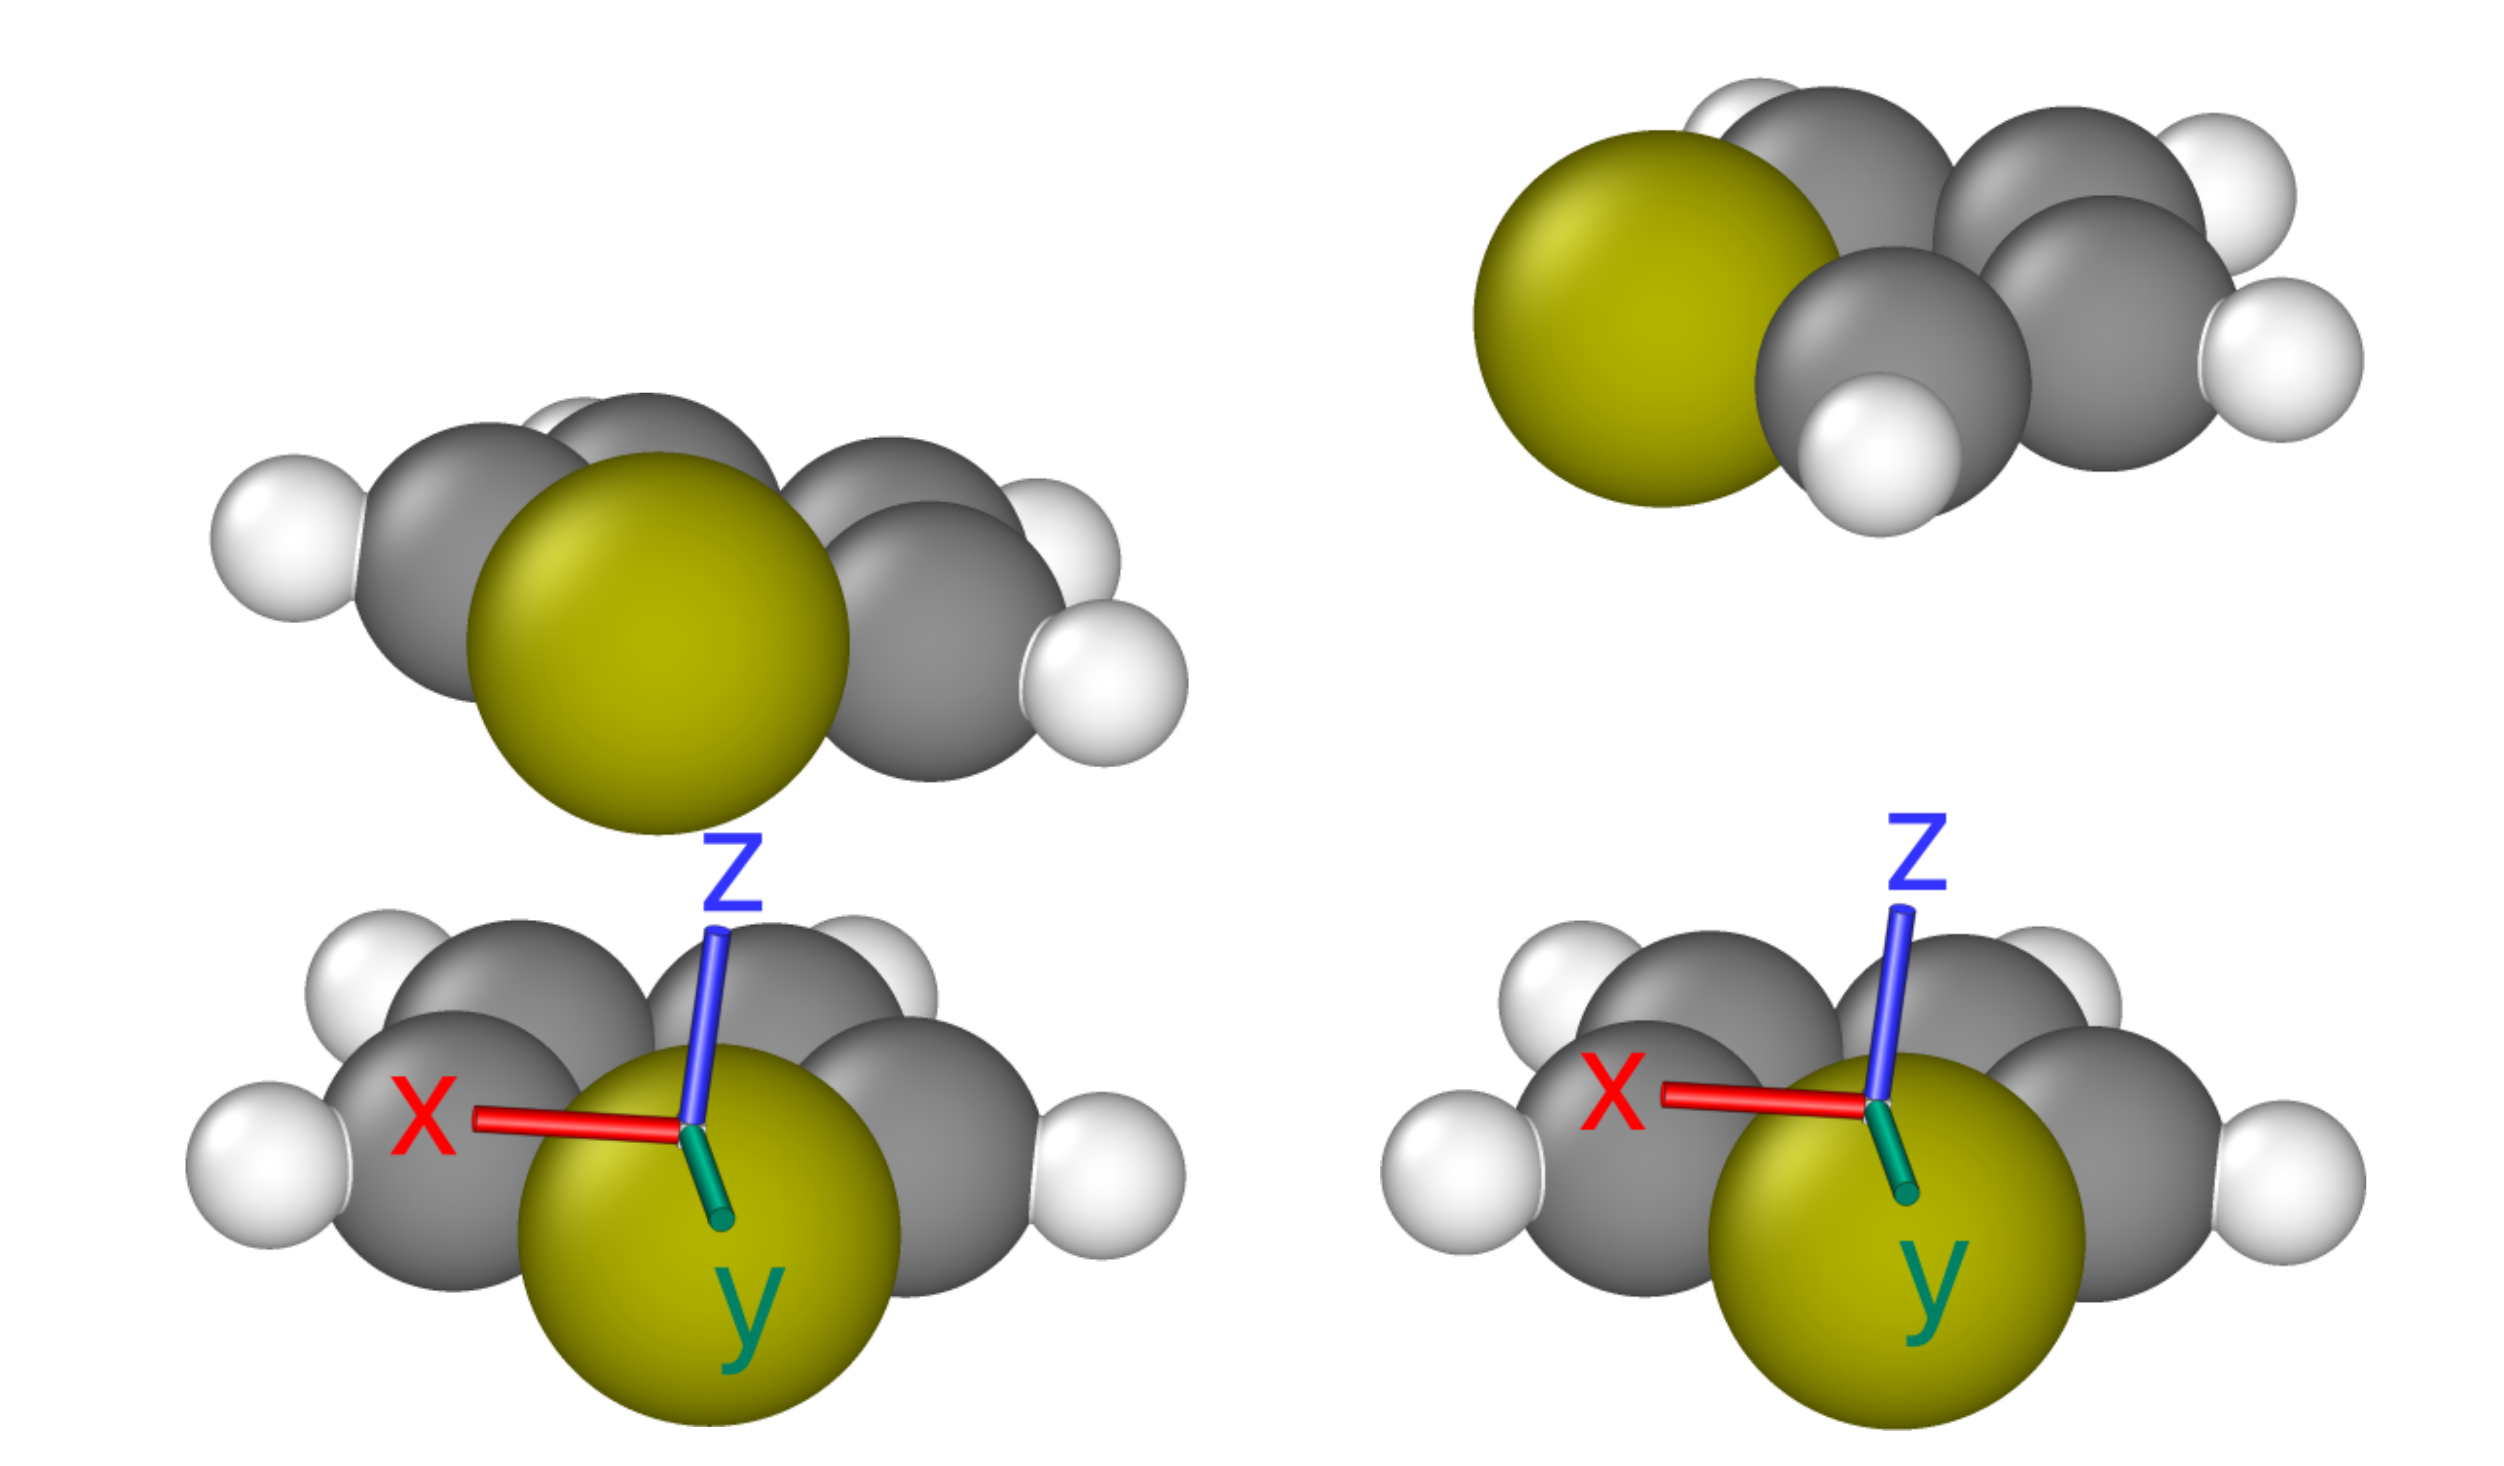
\includegraphics[width=.5\textwidth]{figures/thiophene-oreintations.png}
    \caption{LEFT: The orientation (x-axis rotation ${\sim}0.14$, z-axis rotation ${\sim}-0.14$, center-to-center ${\sim}3.2$)
    with the hightest $T_{ij}$. RIGHT: The orientation (x-axis rotation ${\sim}-0.14$, z-axis rotation
    ${\sim}-1.5$,
    center-to-center ${\sim}5$) with the lowest $T_{ij}$.}
\end{subfigure}%
\caption{ }
\label{TIplots}
\end{figure}

For the orientations found to be most and least optimal we calculate (shown in \autoref{TIplots}),
a $T_{ij}$ of $.00005eV$ and $.15eV$ respectively. In the context of \autoref{marcus} and \autoref{waittime},
the corresponding wait time for a charge to hop between to thiophenes in these orientations is $\tau = 2
\cdot 10^{-14}s$ and $\tau = 2 \cdot 10^{-7}s$. With latter case being two orders of magnitude slower than the
lifetimes allowed in our \glsxtrshort{kmc} simulations, a hop would be highly unfavored for this orientation. 

Creating the directory of \texttt{gsd}s and quantifying the $T_{ij}$ between
them took a wall time of $3.2h$ which averages to ${\sim}2s$ per orientation. 

As evidenced by \autoref{TIplots}((a)), for orientations resulting in a center-to-center distance of less than
$0.5nm$ we calculate an average $T_{ij}$ of ${\sim} 0.28eV$.  
These calculations match closely those
calculated using more rigorous \textit{ab initio} DFT methods\cite{Lan2008},
where realistic distances between thiophene rings in lamellar \glsxtrshort{p3ht} crystals 
between $0.38nm$ and $0.4 nm$ gives $T_{ij}$ values between $0.07eV$ and $0.1eV$. 

In a similar work using a random forest machine learning to predict $T_{ij}$
between thiophenes based on 9 input features, the authors found that the
features of most importance for predicting $T_{ij}$ was bonded vs non bonded,
center-to-center distance and rotation about the y-axis. \cite{Jankowski2019c}

Graduating these pairwise energetics to charge characteristics on the scale of MD simulations
requires the use of an iterative algorithm. For this we employ \glsxtrshort{kmc} simulations using \texttt{MorphCT}.

\subsection{Charge Transport Calculation Validation}

Having explored the performance of \texttt{pySCF} on the level of the molecule, we graduate these computations to the
macroscopic scale with \texttt{MorphCT} to obtain charge mobility.
In a previous work \cite{Miller2018}, researchers used \texttt{MorphCT} to predict charge mobility in \glsxtrshort{p3ht}. 
With \texttt{pySCF} newly integrated into \texttt{MorphCT} for reasons outlined in \autoref{morphct},
we validate our charge mobility against this work.
The benchmark morphologies, which are the final frame of benchmark MD simulations,
used to carry out this validation are public \cite{P3HTData}. 

These benchmark simulations were carried out using coarse-graining techniques
wherein molecular segments have been unified and treated as individual beads to lower
computational cost and allow for larger and longer simulations. 
Using the Optimized Potentials for Liquid Simulations United Atom (OPLS-UA) force field,
the researchers ran united-atom simulations, which do
not explicitly keep track of the hydrogens in the simulation, 
but nevertheless accurately predict equilibrium geometries. This allowed the researchers to access length scales
at which individual grains can form within the morphology. The orientation and boundaries of these grains effect
charge transport and therefore provide a critical benchmark to compare against. 

We first fined-grained MD data (hydrogens appended back into
the morphology) and converted from \texttt{xml} to \texttt{gsd} format. At
current, \texttt{MorphCT} is compatible with all-atom data and \texttt{gsd} format. 
As visualized in \autoref{molecules}, chromophores are taken to be individual monomers. 
Using \texttt{MorphCT}, for each chromophore, a unique object is instantiated and the energetics are obtained using
\texttt{pySCF}. A \glsxtrshort{kmc} simulation is performed on the basis of these energetics with \glsxtrshort{kmc} temperature set to 300K. For
each morphology, 10,000 individual charge carriers are injected (one at a time) into the morphology, with
5,000 restricted to a lifetime of a tenth of a nanosecond and 5,000 restricted
to a lifetime of a nanosecond.
As outlined in \autoref{kmcanalysis}, from the difference in \glsxtrshort{msd}
between these sets of charge carriers, the
zero-field charge mobility for the morphology is obtained. 

\begin{figure}
  \center
  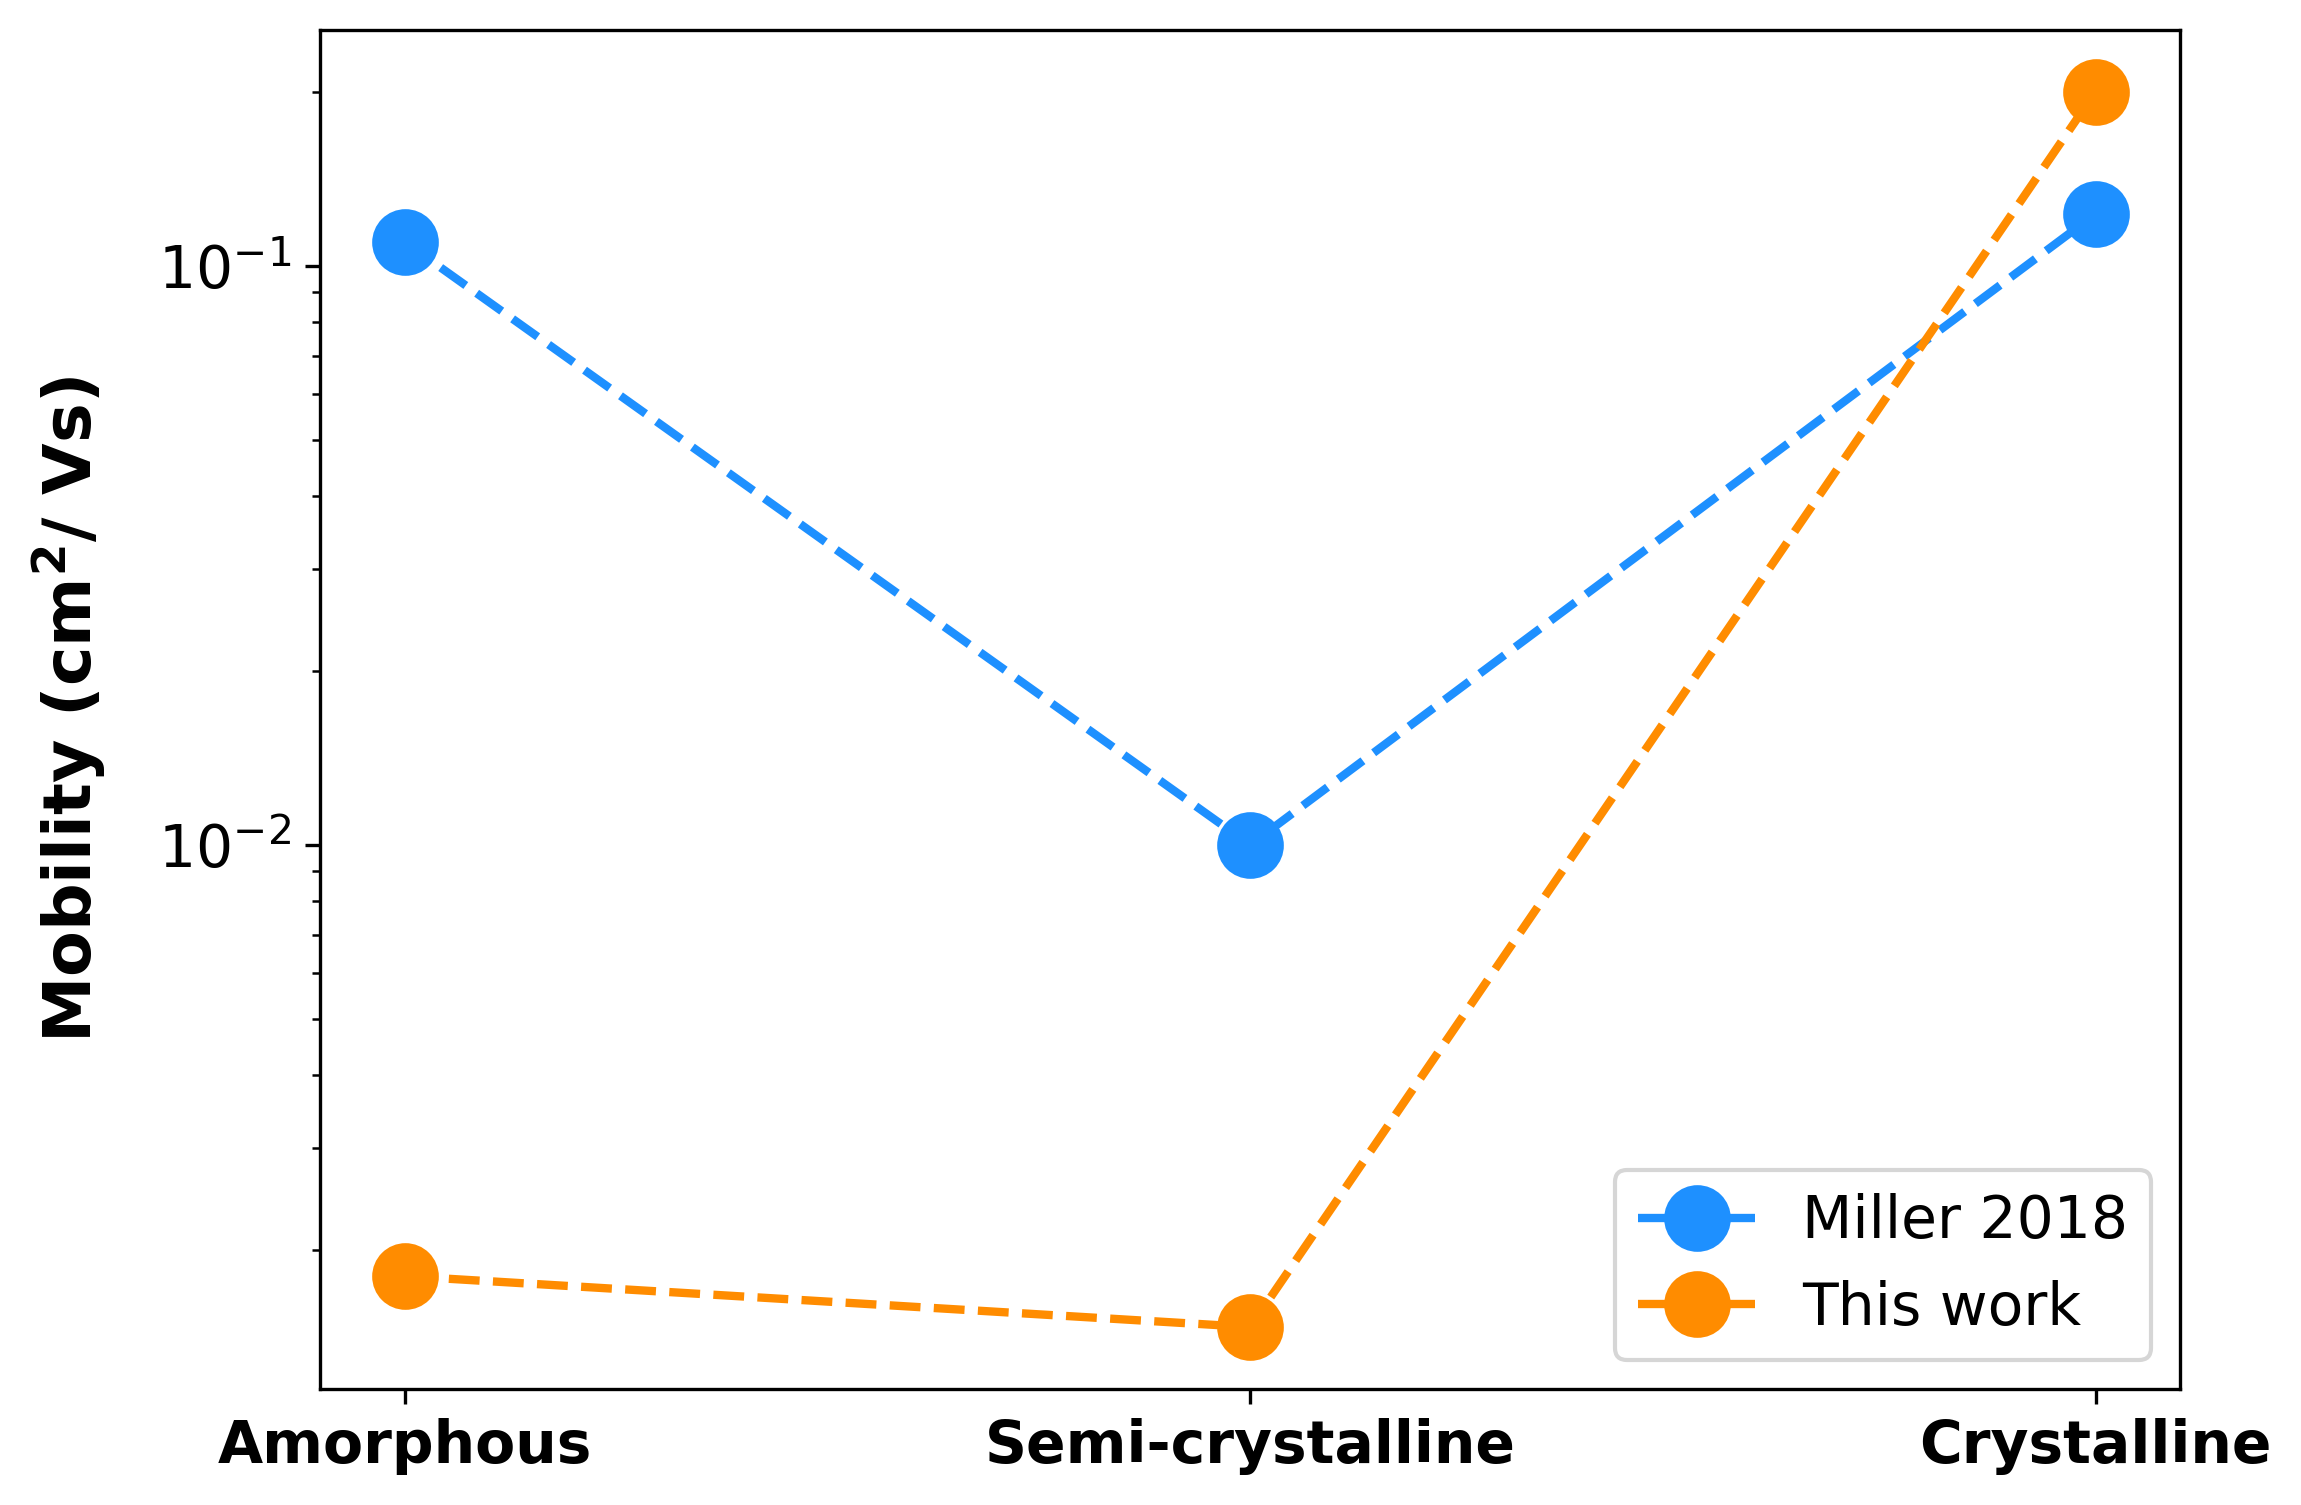
\includegraphics[width = .6\textwidth]{figures/validation.png}
  \caption{The results of mobility prediction on benchmark \glsxtrshort{p3ht} mobilities. We report the data in this way to
    show that the we found the same trend as previously reported using \texttt{ORCA} for \gls{qcc}s. }
  \label{mobility-validation}
\end{figure}

It is known about \glsxtrshort{p3ht} that it can have vastly different crystallinities based on how it has been processed. 
We validate on three morphologies with crystallinities that vary from amorphous
to highly crystalline. These morphologies have been coerced into various levels
of crystallinity through a simulated annealing process. 
We refer to these morphologies as disordered, semi-crystalline, and crystalline.

Results from our work compare well to a predecessor of our work, which implemented ZINDO/s, another
semi-empirical \glsxtrshort{qcc} method \cite{Miller2018a}\cite{Jones2017}. 
Their work utilized an earlier version of \texttt{MorphCT} which used the \glsxtrshort{qcc} software 
\texttt{ORCA} \cite{Neese2012b} to provide the quantum chemical approximations. 
\texttt{ORCA}'s proprietary licensing was prohibitive in the efforts to containerize \texttt{MorphCT} for use on cluster and for
creating reproducible results. This motivated the restructuring of \texttt{MorphCT} for use with \texttt{pySCF}. The
performance of \texttt{pySCF} and of the current \texttt{MorphCT}.

The results in \ref{mobility-validation} show the charge mobility reported in the prior work, which used \texttt{ORCA} for
the \glsxtrshort{qcc} calculation, and the charge mobility obtained using using the current workflow, which uses \texttt{pySCF}. 
The previous work found that charge mobility is highest for the crystalline morphology, followed by the
amorphous, and finally the semicrystalline. This seemingly anomalous behavior can be explained. While the
semicrystalline morphology has more ordered high speed highways of transport, the anisotropic movement
inhibits average displacement. Our work replicates this trend.

In the previous work on these \glsxtrshort{p3ht} morphologies, 7 lifetimes were chosen and a linear regression was performed
to estimate the slope of the \glsxtrshort{msd}. The current work found that the mobility can be appropriately reproduced
with an appropriate choice of 2 lifetimes beyond the ballistic transport timescale. It was found that with the 
squared displacement averaged over 5000 holes at $10^{-9}s$ and again $10^{-10}s$ the slope of the \glsxtrshort{msd} can be reproduced with 1000's less individual holes having to be simulated.

\section{Charge Transport Sensitivity Analysis}

\label{sensitivity}

The sensitivity of our \gls{kmc} simulation analysis to various parameters was performed on the benchmark 
crystalline \glsxtrshort{p3ht} morphology. As the overarching goal is to
connect the morphological features to charge mobility, it is critical to be
explicit about how each parameter can affect the resulting value of charge
mobility. 

By pressure testing the algorithm with a range of values for our input
parameter, we explore the robustness of the algorithm to individual inputs.
Sensitivity analysis can also help us understand where to
invest resources into dialing
the accuracy of any given parameter. It also gives motivation to be meticulous about keeping these parameters
constant across analysis of the same material under different processing conditions. For example, if a higher
charge mobility is discovered for a given morphology after some simulated annealing,
it should be confirmed that it is not because the researcher used a lower reorganization energy for example. 

We perform sensitivity analysis for $4$ parameters: (1) neighbor cutoff
distance ($d_{cut}$), (2) chromophore reorganization energy, (3) \gls{kmc}
temperature, and (4) choice of carrier lifetimes. 

\subsection{Neighbor Cutoff ($d_{cut}$)}
\label{dcutresults}
Voronoi analysis allows for the computationally efficient partitioning of space into
polyhedra chromophore cells. As shown in \ref{fig:dcut}, chromophore $i$ is the neighbor of chromophore $j$
if the voronoi cells constructed around their geometric center
share a boundary with one another. 

With each chromophore pair requiring a relatively costly \glsxtrshort{qcc}, after narrowing down the chromophore pairs with voronoi, it
could be
computationally preferable to calculate the distances between all pairs and remove neighbors more than $d_{cut}$
apart.

\begin{table}
\caption{$d_{cut}$ Sensitivity}
\centering % used for centering table
\begin{tabular}{c c c c c c c c} % centered columns (4 columns)
\hline\hline %inserts double horizontal lines
    $d_{cut}$ $\text{\AA}$ & 4 & 6 & 8 & 10 & 12 & 14 & 16 \\ [0.5ex] % inserts table
%heading
\hline  % inserts single horizontal line
pairs & 318 & 22000 & 49000 & 96000 & 113026 & 113315 & 113315 \\ [1ex]% inserting body of the table
$\mu_{0}$ $(cm^{2}/Vs)$ & $-2.17 \cdot 10^{-6}$ & $6.13 \cdot 10^{-4}$ & .01 & .17 & .17 & .22 & .22 \\ [1ex] % [1ex] adds vertical space
%$\mu_{0}$ Error & $-1.75*10^{-6}$ & 6 & 8 & 10 & 12 & 14 & 16 \\
\hline %inserts single line
\end{tabular}
\label{table:dcut-sense} % is used to refer this table in the text
\end{table}

\autoref{table:dcut-sense} shows the effect of cutoff distance on value of
calculated mobility.  
 We can see in table \ref{table:dcut-sense}, that with $d_{cut}=10$ we get comparable mobilities to the
$d_{cut}$ 12 simulation with $10^5$ less
pairs, which could suggest that beyond $d_{cut}$ 10 there is a diminishing returns on mobility prediction with the
additional chromophores. 

However, we found for the materials currently under investigation,
\texttt{pySCF} is speedy enough such that introducing $d_{cut}$ adds more ambiguity
into the workflow than is necessary given that the average time per \glsxtrshort{qcc} dimer calculation is .036s for \glsxtrshort{p3ht} and
1.2s for \glsxtrshort{itic}. Furthermore, with \texttt{MorphCT} acting on static atomistic orientations, these calculations 
are only necessarily performed once per morphology. With that, our workflow defaults this cutoff distance to half
the length of the simulation box, rendering it effectively moot. 

If, in the future, more computationally expensive methods are incorporated into the \glsxtrshort{qcc} step, or chromophores in other
organic materials are a heavier lift \texttt{pySCF}, it could be beneficial to reintroduce this cutoff distance. The optimal $d_{cut}$ will vary depending on the material and before doing large sweeping analysis on a new
material its at a discount to do some preliminary analysis to determine an appropriate value. We tested the
sensitivity of the algorithm to the value ($d_{cut}$). 

\subsection{Reorganization energy}

In the context of \autoref{marcusmodel}, 
reorganization energy, $\lambda_{ij}$, constitutes the energy required to distort the dimer's equilibrium geometry with a
charge on chromophore $i$ into the dimers equilibrium geometry with charge on chromophore $j$.
Reorganization energy consist of the energy change associated with the distortion of the dimers geometry,
and the distortion of the surrounding medium in response the movement of the charge. It can be written as
follows:
\begin{align}
    \lambda_{total} = \lambda_{internal} + \lambda_{external}.
\end{align} 
$\lambda = 0.3eV$ is chosen to be the default reorganization energy ($\lambda_{internal} = 0.1eV$
and $\lambda_{external} = .02eV$) as others have done with \glsxtrshort{p3ht} \cite{Jones2017} and
a flourene-triphenylamine copolymer, TFB \cite{Gali2017}. 

\begin{figure}
\centering
\begin{subfigure}{\textwidth}
    \textbf{(A)} \\
    \centering
    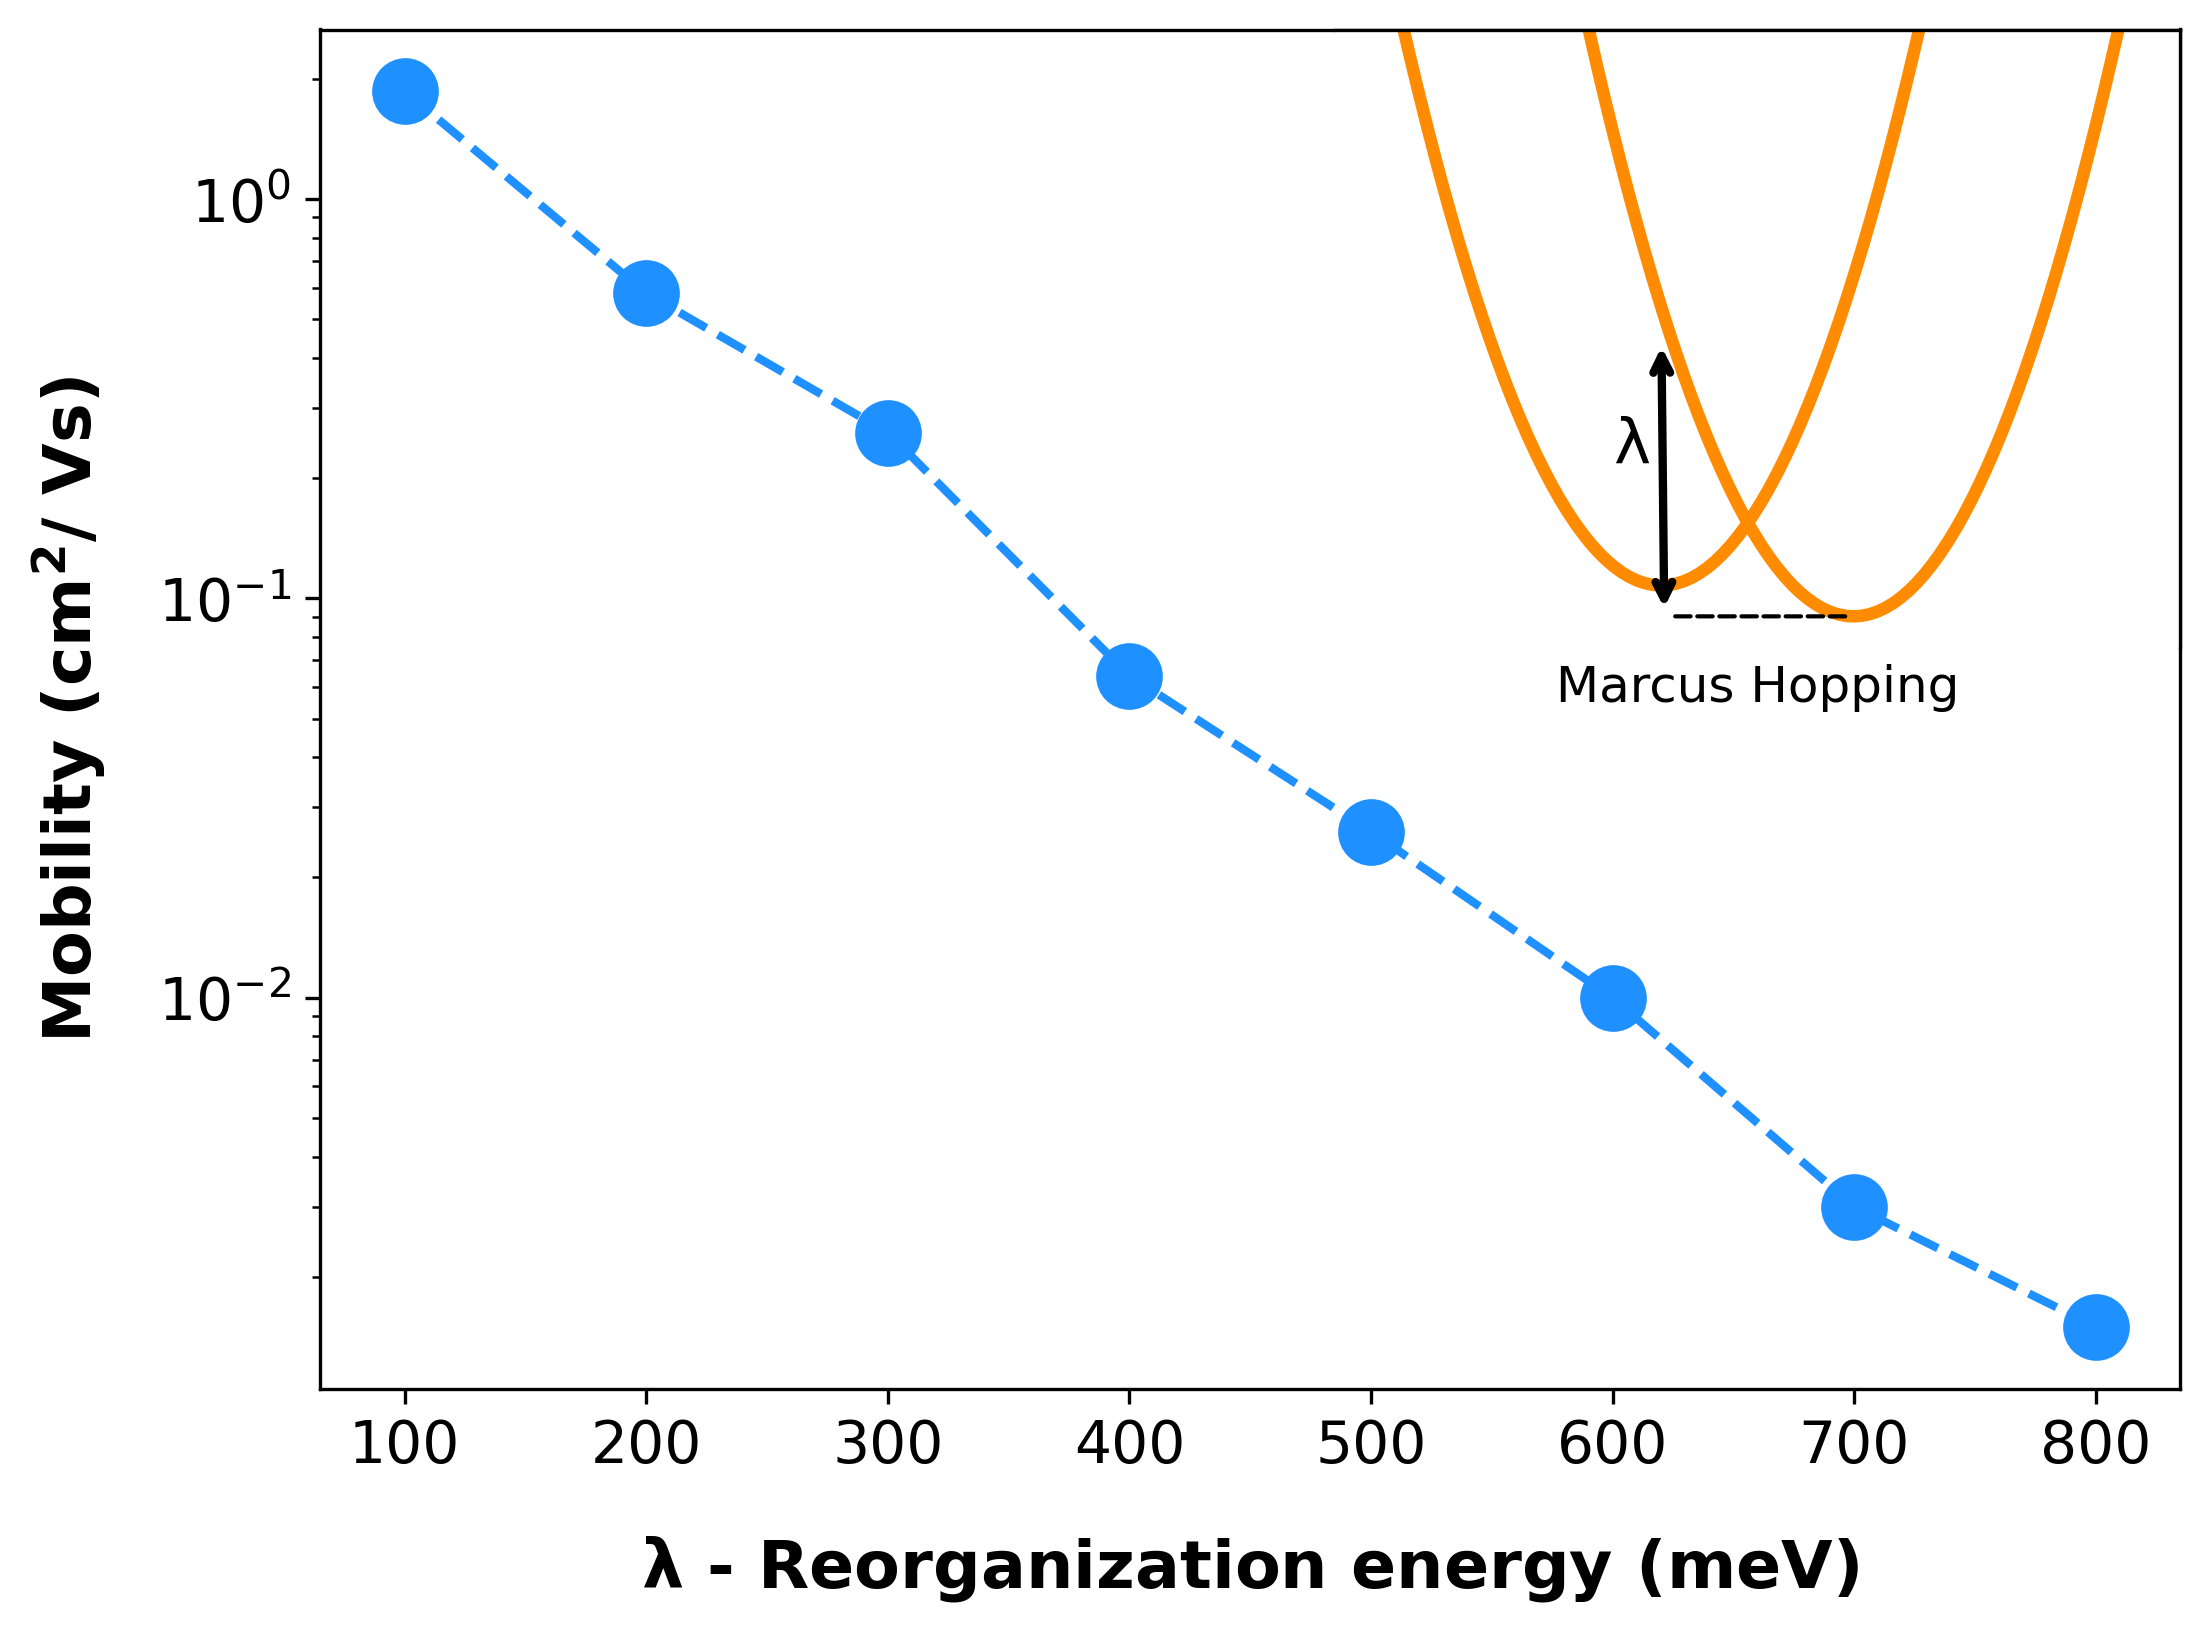
\includegraphics[width=.8\textwidth]{figures/reorg-log-yaxis.png}
    \newline
\end{subfigure}%
\\
\begin{subfigure}{.5\textwidth}
    \textbf{(B)} $\lambda = 100$
    \centering
    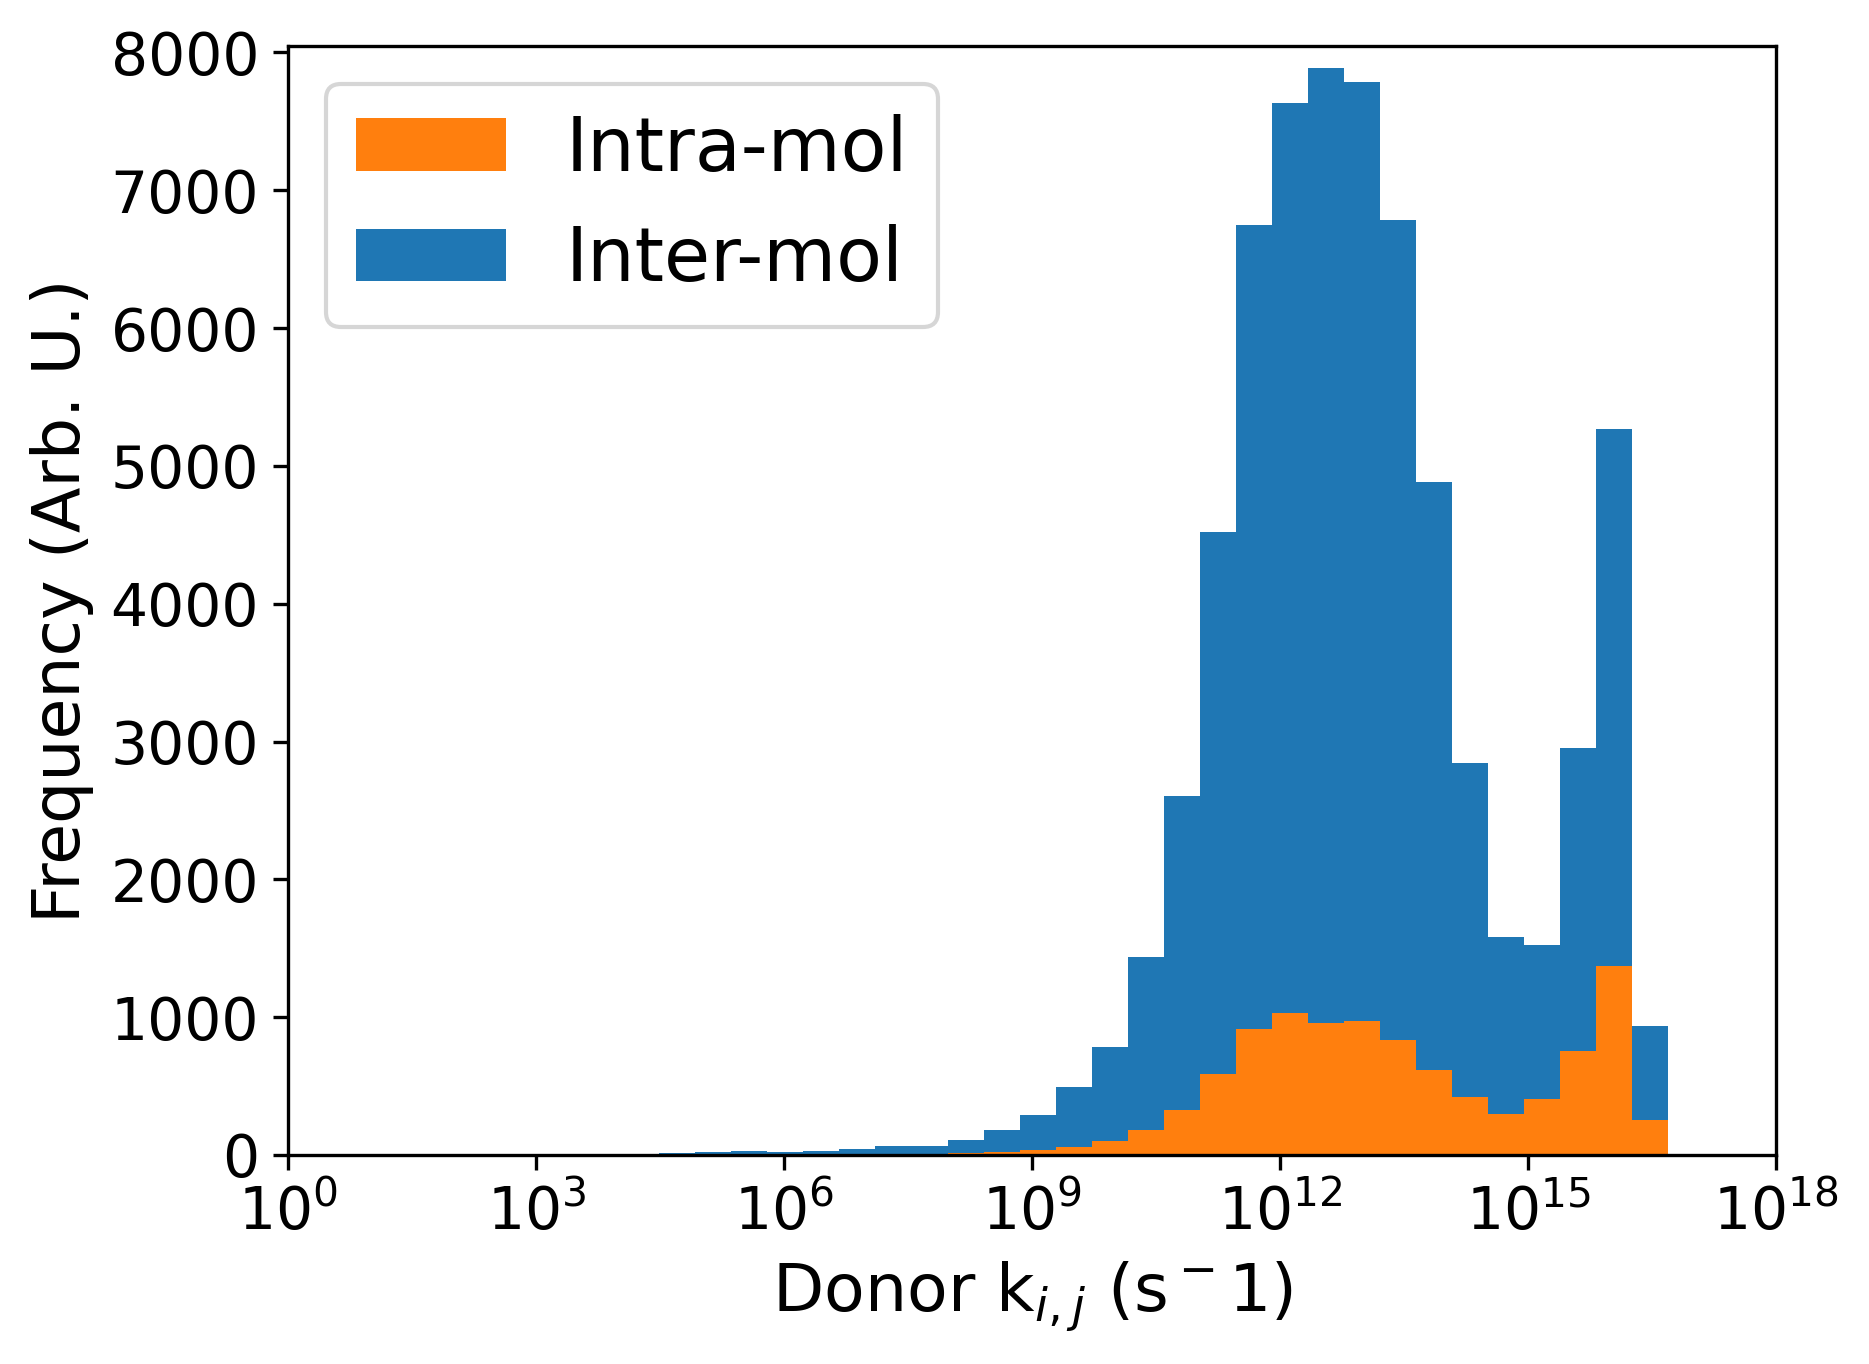
\includegraphics[width=\textwidth]{figures/donor_hopping_rate_clusters_reorg100.png}
\end{subfigure}%
\begin{subfigure}{.5\textwidth}
    \textbf{(C)} $\lambda = 800$
    \centering
    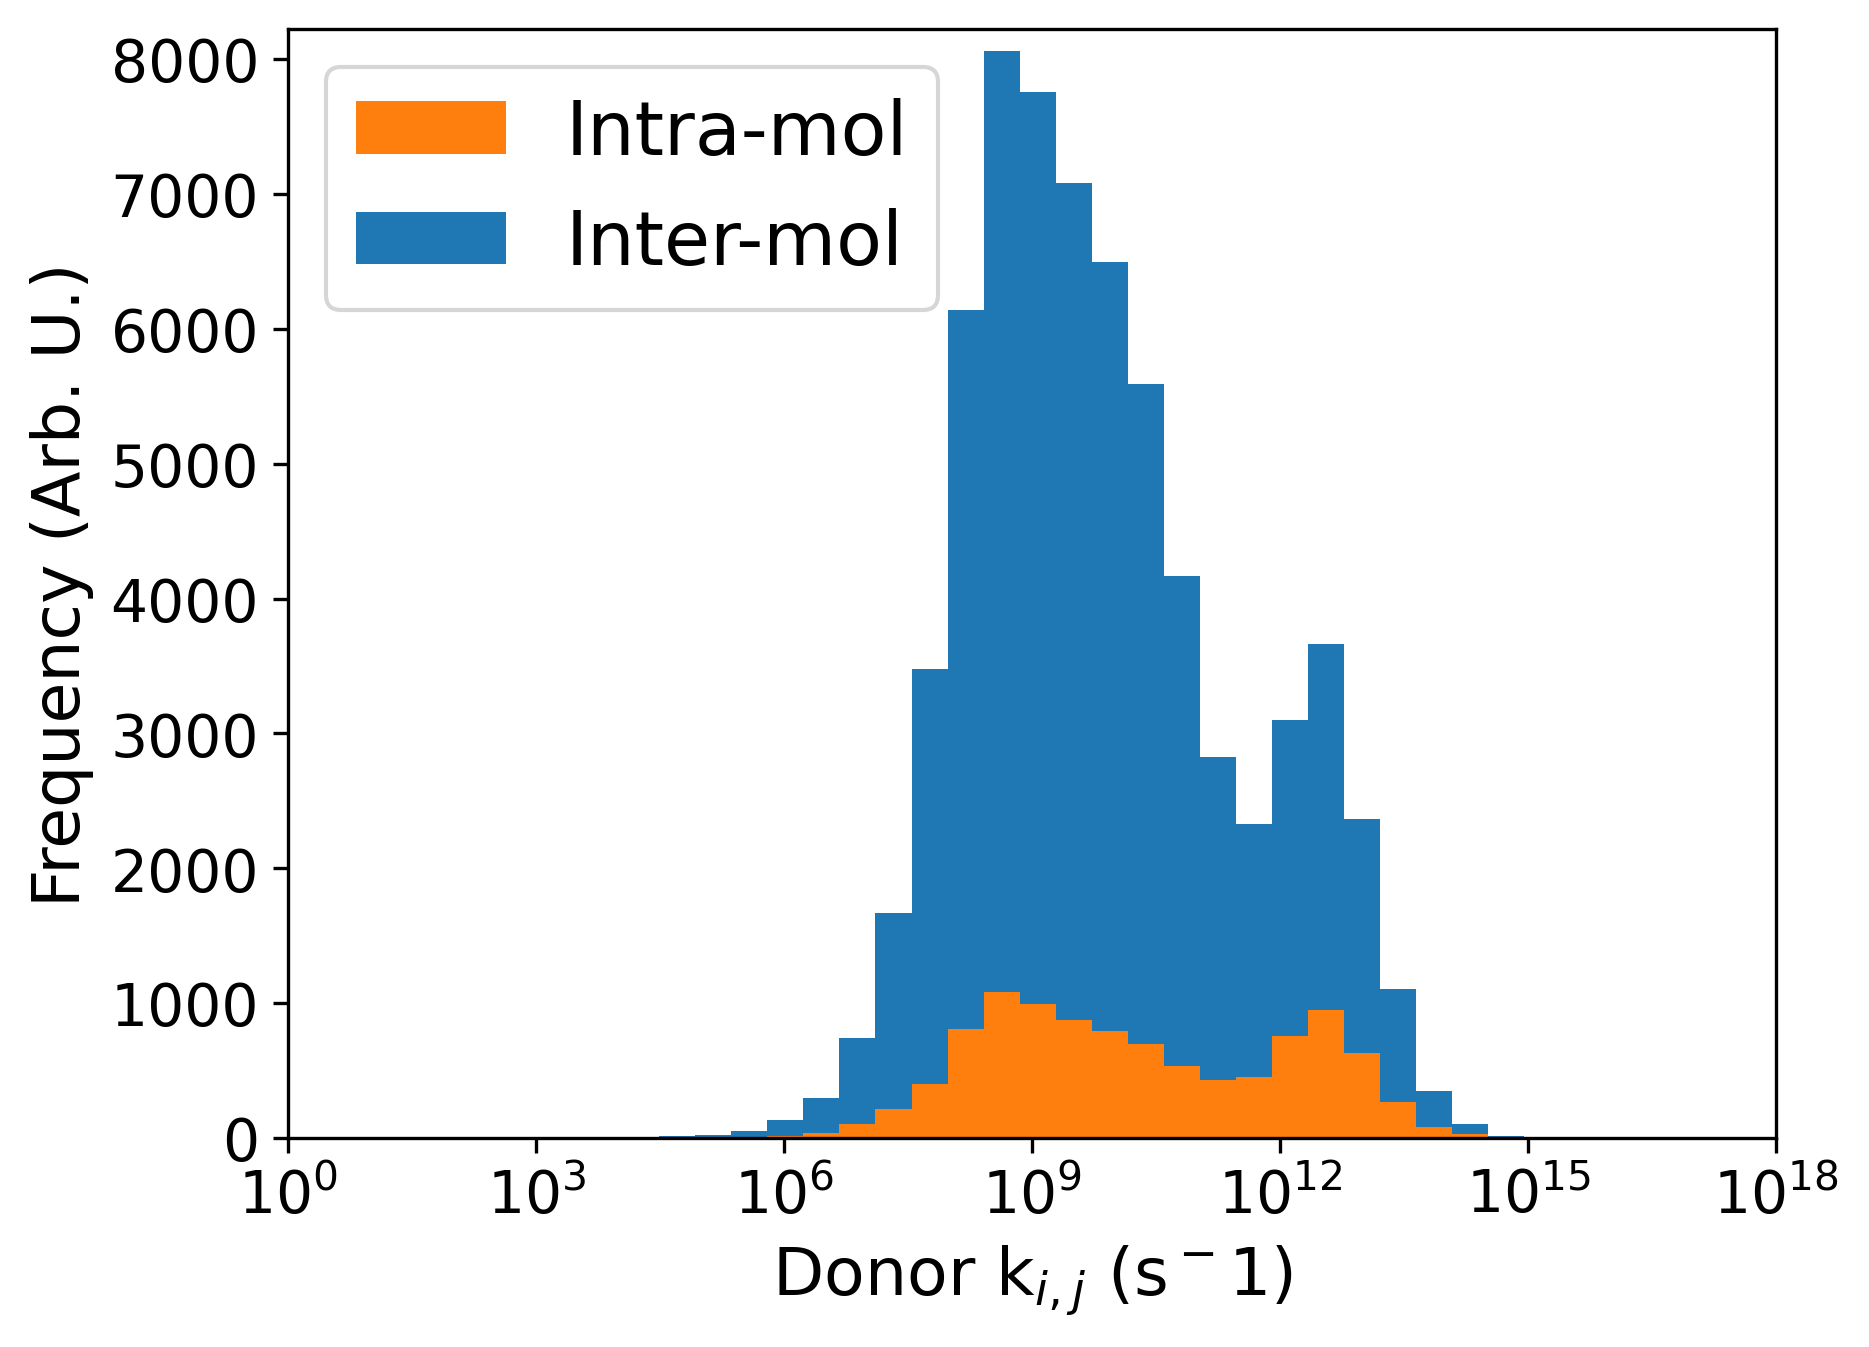
\includegraphics[width=\textwidth]{figures/donor_hopping_rate_clusters_reorg800.png}
\end{subfigure}
    \caption{Figure (A) shows how \glsxtrshort{kmc} simulated mobility values scale with the prescribed
    reorganization energy values, $\lambda$. Figures (B) and (C) show the distribution of hopping rates with
    $\lambda = 100eV$ and $\lambda = 800eV$ respectively. We see that the exponential decay of charge mobility as
 reorganization energy increases is a result of a shift in the distribution of hop rates throughout the
    simulation.  
    }
\label{reorg}
\end{figure}

In our workflow, reorganization energy is set as an attribute
to the chromophore object. It is defaulted to ${\sim}300meV$ as for all chromophore
objects.
To test the sensitivity of the algorithm to this value we ran $8$
simulations with chromophores assigned reorganization energies of $100-800meV$.
In \texttt{MorphCT}, this is as easy as retrieving the pickled crystalline system, looping through the chromophores, setting the
reorganization energy, and rerunning the \gls{kmc} simulation. 

The results, shown in
\autoref{reorg}, are expected from the inspection of \autoref{marcus}. Because these simulation were run on
the same morphology, the variation in distributions of $k_{ij}$ values, shown in \autoref{reorg}(B)(C), is
solely due to the choice of $\lambda$. The cumulative outcome of this is the exponential decay in mobility as
$\lambda$ is increased.

\subsection{Temperature}

\begin{figure}
\centering
\begin{subfigure}{.5\textwidth}
    \textbf{(A)}
    \centering
    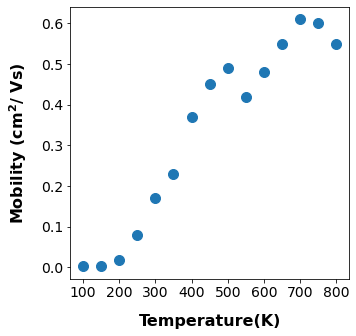
\includegraphics[width=.9\textwidth]{figures/temp.png}
    \newline
\end{subfigure}%
\begin{subfigure}{.5\textwidth}
    \textbf{(B)}
    \centering
    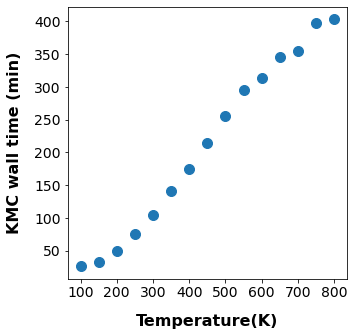
\includegraphics[width=.9\textwidth]{figures/temp_simtime_plot.png}
    \newline
\end{subfigure}
\begin{subfigure}{.5\textwidth}
    \textbf{(C) 100K}
    \centering
    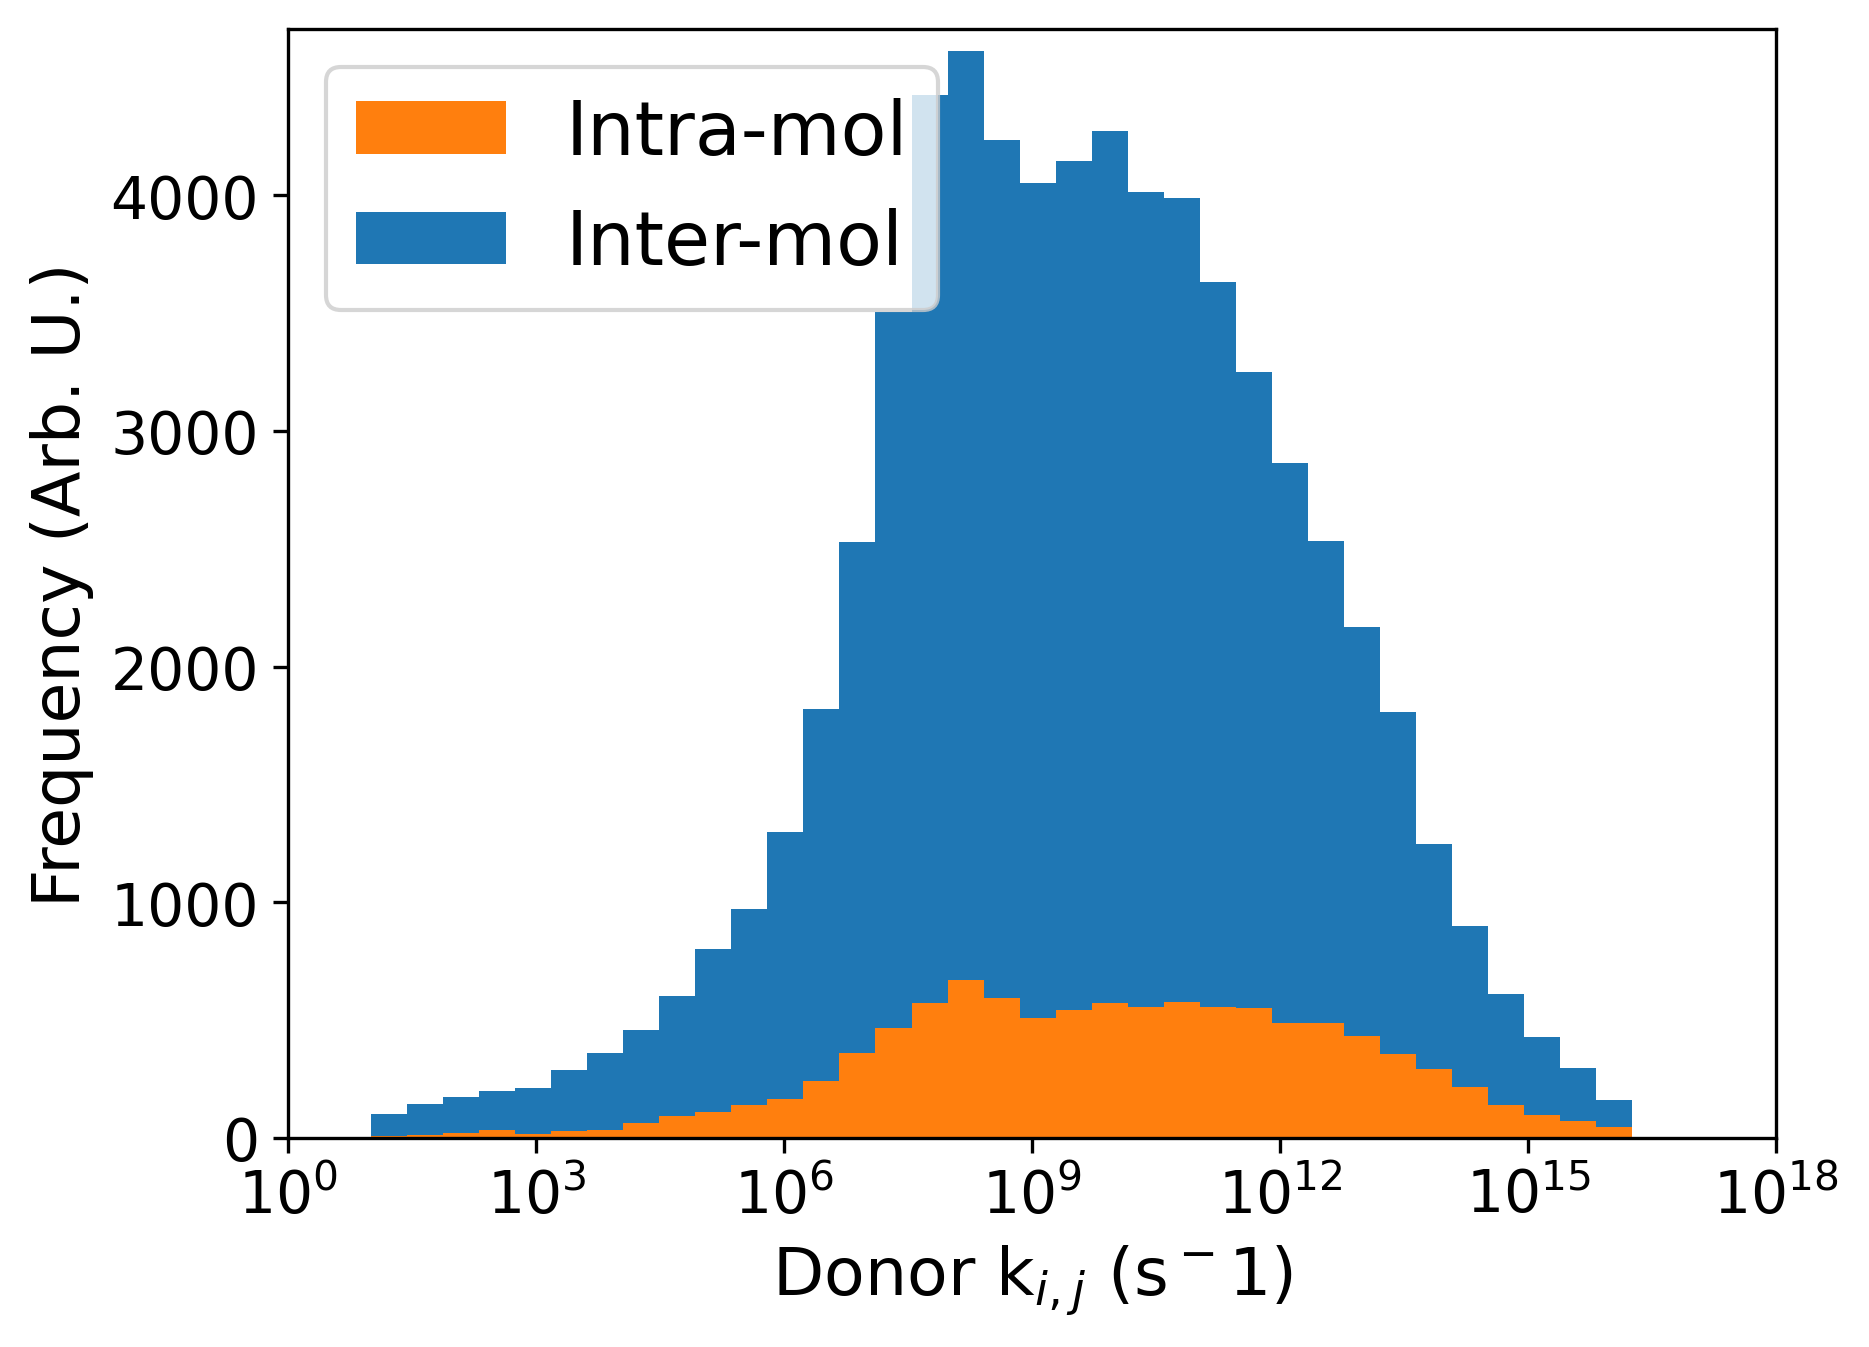
\includegraphics[width=\textwidth]{figures/donor_hopping_rate_clusters_temp100.png}
\end{subfigure}%
\begin{subfigure}{.5\textwidth}
    \textbf{(D) 800K}
    \centering
    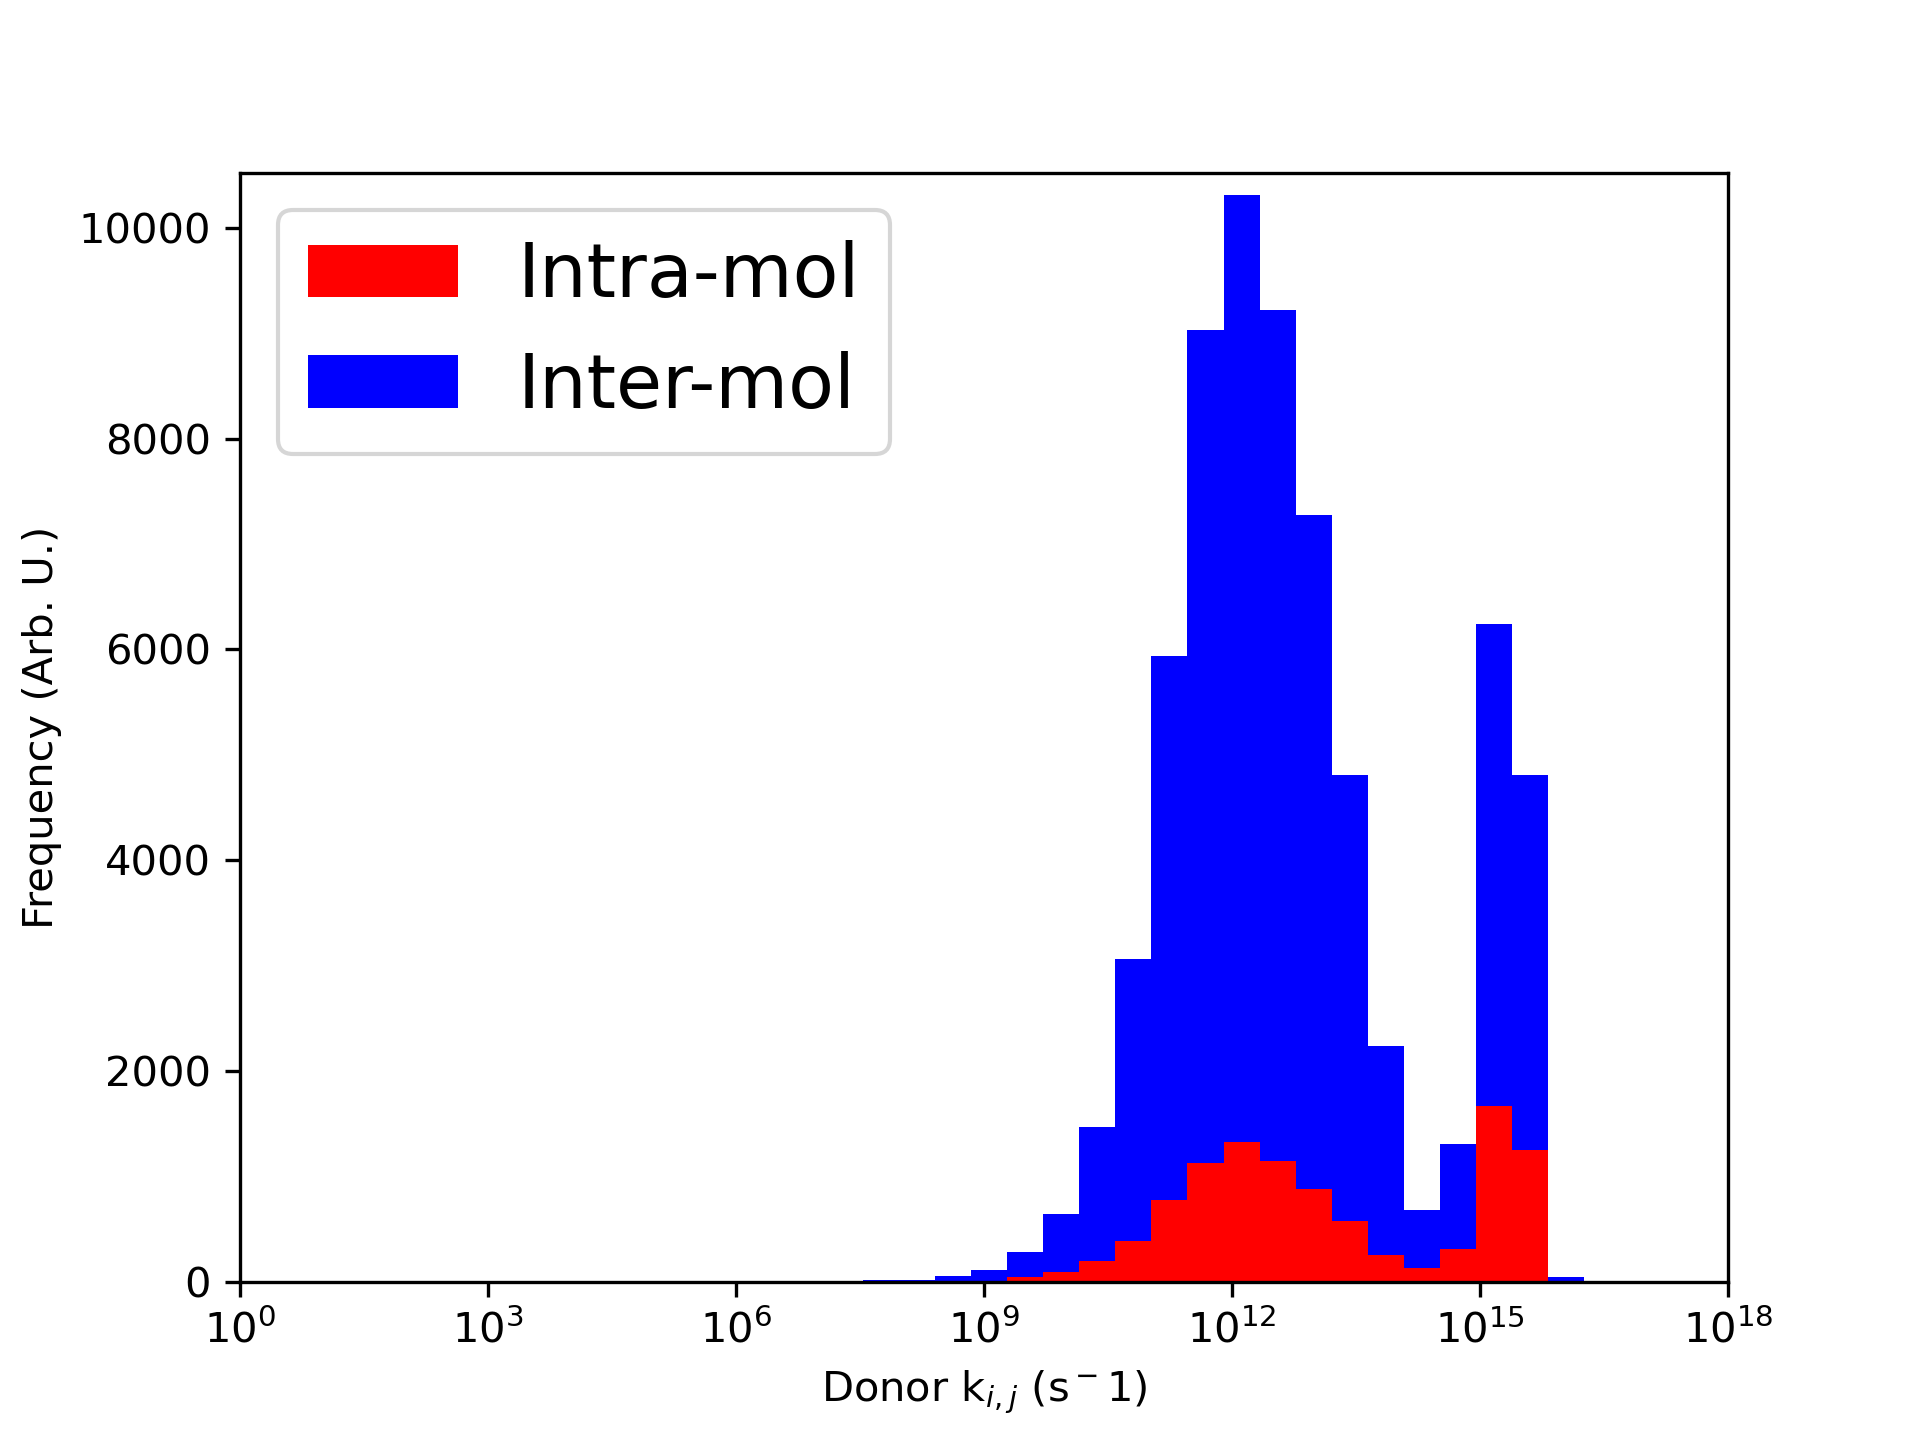
\includegraphics[width=\textwidth]{figures/donor_hopping_rate_clusters_temp800.png}
\end{subfigure}
    \caption{The resulting mobility (A) and \gls{kmc} wall time (B) of 15 \gls{kmc} simulations from $100K$ to
    $800K$. The hop rate distribution for the lowest (C) and highest (D) temperature \gls{kmc}
    simulations are provided as context for the relationships observed in (A) and (B).
    With each hop modeled as a thermally
    activated process, an increase in temperature increases average hop rate and mobility. Orders of
    magnitude faster hops means orders of magnitude more hops to track in computer memory over a charge
    carrier's lifetime, which we see results in longer \gls{kmc} simulation wall times.}
\label{TEMP}
\end{figure}

To test the sensitivity of our implementation to
temperature, $15$ \glsxtrshort{kmc} simulations from $100K$ to $800K$ were run on the benchmark \glsxtrshort{p3ht} crystalline morphology. It is clear from the results in figure \ref{TEMP}(A) that the mobilities trend upward with temperature.
This should be expected from the assumptions of the model outlined in \autoref{marcusmodel}. 
With relatively weak electronic coupling ($T_{ij}$) between chromophores, electron transfer proceeds nonadiabatically \cite{clarke2010}. With this weak coupling, the temperature in the Gibbs free energy of activation term
dominates the effect that temperature has on the hop rate value calculated with \autoref{marcus}.

An interesting result is that increasing the temperature of the \glsxtrshort{kmc}
simulation also increases the wall time of the \gls{kmc} simulations.
As an illustration of why this is the case, the distribution of hop
rates is plotted for $100K$ and $800K$ in figure \ref{TEMP}(C)(D). With the distribution of hop rates skewed
drastically higher at $800K$, each charge carrier will experience orders of
magnitude more hops during its specified lifetime. 

\subsection{MSD (lifetimes)}

Introduced in \autoref{kmcanalysis}, the `carrier lifetimes' chosen for a given
simulation can effect the analysis of the slope of the \gls{msd} as time goes
to infinity. 
Including \gls{msd} data for an extremely short lifetime can inflate
the estimation. Including \gls{msd} data for extremely long lifetimes wastes computation and could introduce unnecessary noise into the data \cite{Maginn2018}. 
For example, in an attempt to simulate out to the physical limit, a
simulation with a microsecond($10^{-6}s$) lifetime resulted in a single hole hopping for 9 wall time hours.

In real systems, free charge
carrier lifetime is subject to a complex interplay between geminate recombination, non-geminate recombination,
charge trapping, temperature, and charge density. These dynamics play out across a picosecond to microsecond
timescales and vary wildly form material to material and from microstructure to microstructure for a
given material \cite{Laquai2015}.

Testing the sensitivity of this choice was not as one-to-one as it was for the
parameters tested above. We could choose as many lifetimes across whatever
length scales we please. We saw that the choice of two lifetimes is sufficient
for estimating slope in \autoref{validation}. So we test the sensitivity to
setting the first lifetime progressively shorter. 

\begin{figure}
  \center
  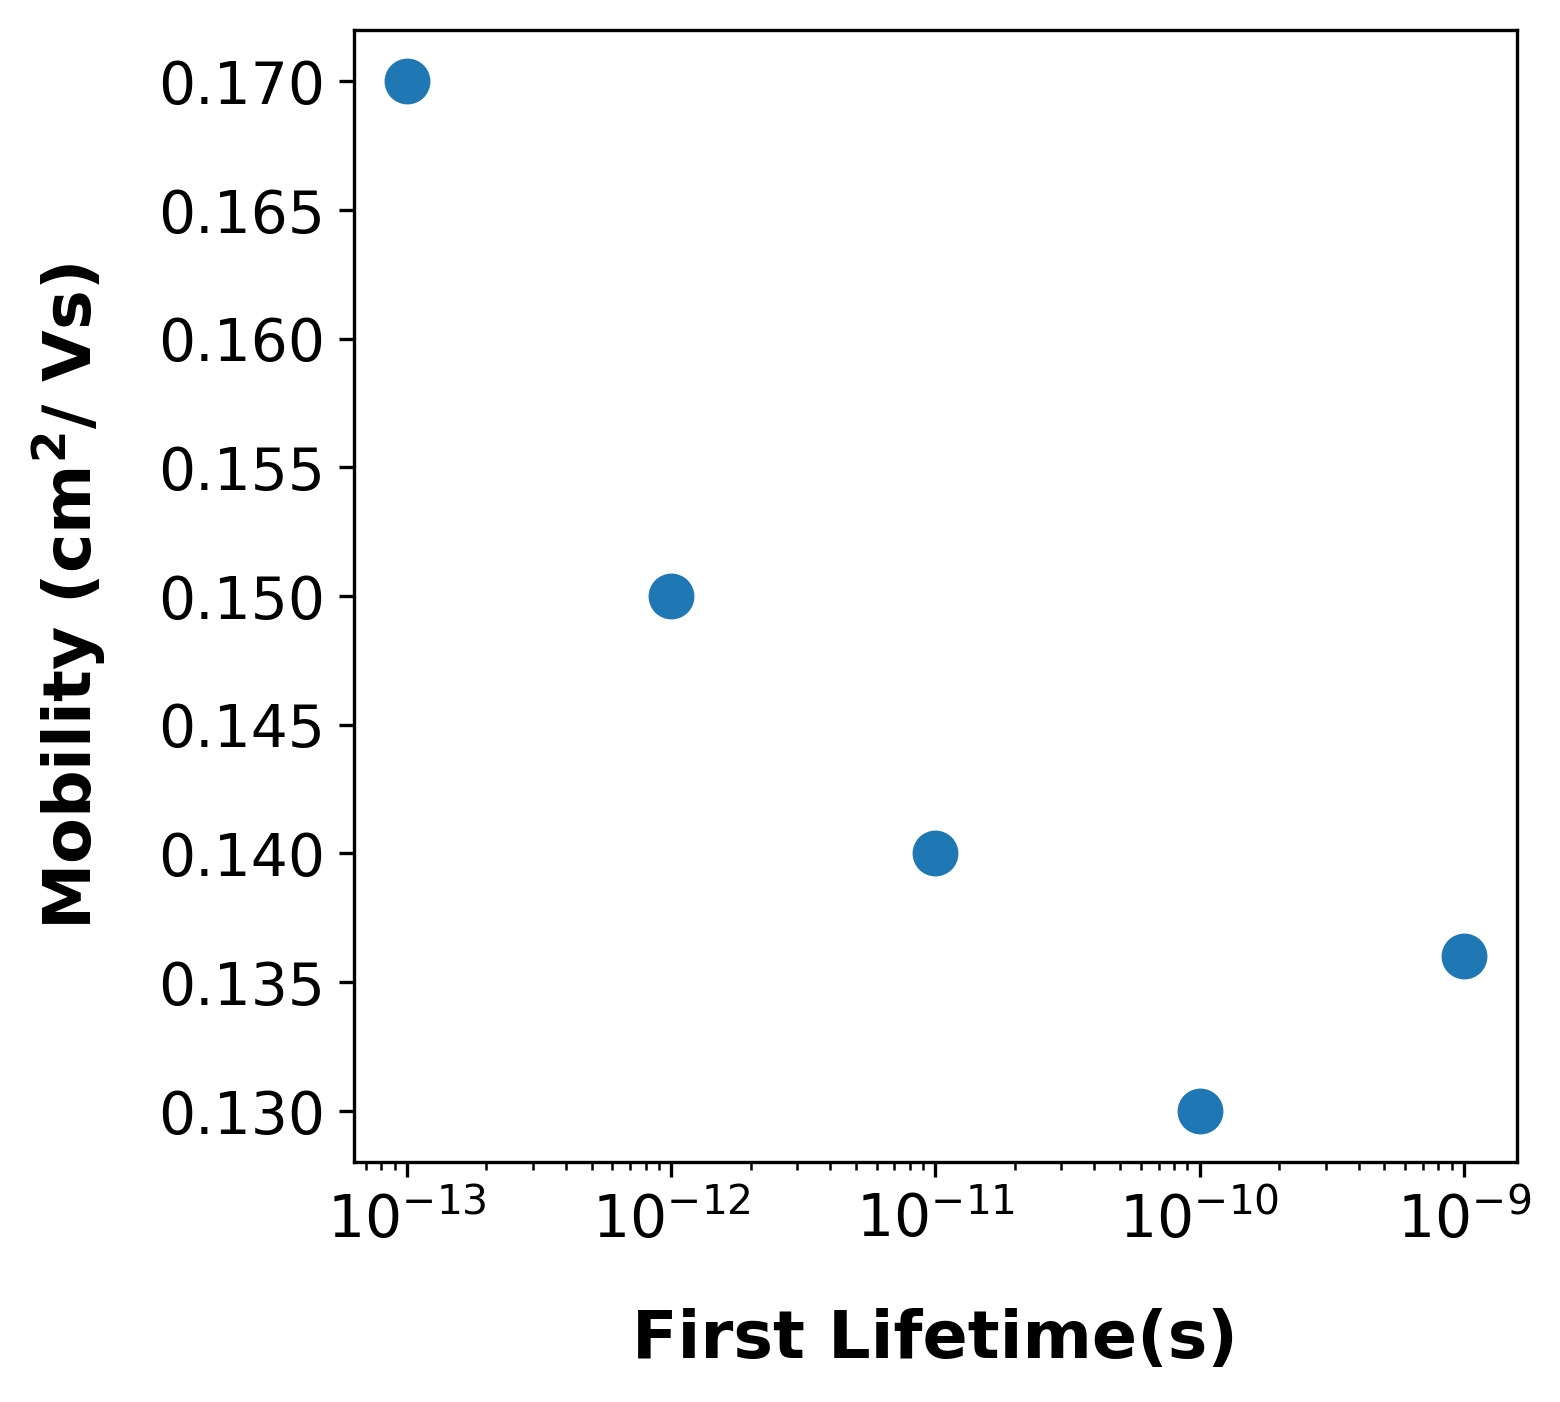
\includegraphics[width=0.6\linewidth]{figures/lifetime.png} 
    \caption{The results of running 5 \glsxtrshort{kmc} simulations with the first lifetimes as described in the text. It
    can be seen that below the ballistic timescale (${\sim}10^{-10}s$), the
    resulting mobility increases.}
  \label{lifetime}
\end{figure}

To do so, we set the second lifetime comfortably in the linear region of the
\gls{msd}. 
In a previous work on \gls{p3ht}, the slope becomes linear around a tenth of a
nanosecond \cite{Jones2017}. With that, we take the second life time to be two
orders of magnitude beyond that at ten nanoseconds.
$6$ simulations were run with progressively shorter first lifetimes.
The first lifetime was set to $10^{-9}s$, $10^{-10}s$,
$10^{-11}s$, $10^{-12}s$, and $10^{-13}s$ respectively. The results are plotted in figure
\ref{lifetime}. 

As expected, as the first lifetime progresses in the ballistic transport
timescale, the resulting mobility increases. If the starting lifetime is even shorter the
workflow breaks down because as can be seen from the hop rate distribution in figure \ref{TEMP}(D), even at
extreme temperatures, holes need more time that that to hop even once.

Interestingly, the algorithm seems to be quite robust against choice of lifetimes. As can be seen in the
figure, order of magnitude differences in lifetime choices results in less than 2X difference in the resulting
mobility. Furthermore, as we saw on \autoref{validation}, fitting the slope of
the \gls{msd} from only two lifetimes results in a satisfactory charge prediction.
This suggests that going lifetime crazy is a waste of computation. What is more
important then is reporting the lifetimes used in the study for comparison
across multiple studies. 

\section{ITIC}

\label{itic}

Our pipeline is meant to facilitate the computational screening of \gls{opv}s.
Here we use the pipeline to predict charge mobility in \gls{itic}.
This is a first foray into the extensibility of the complete pipeline to a
material not named \gls{p3ht}. 

The \glsxtrshort{itic} morphology was simulated using Plankton-Flow \cite{cmelab} on Fry,         
a high performance computing cluster at Boise State University.  
Using \texttt{planckton-flow}, a 1000
molecule morphology of \glsxtrshort{itic} was equilibrated over a $10^{7}$ 
step MD simulation at room temperature. 
From the results of the ${\sim}200nm^{3}$ MD simulation, the last frame of the atomic
trajectories is taken to represent an accurate equilibrium geometry
of \glsxtrshort{itic}. 

To apply the hopping model to this atomistic morphology requires the
delineation of segments within the morphology upon which charges can delocalize along \glsxtrshort{lumo} (or 
\glsxtrshort{homo} for donors).   
The \glsxtrshort{lumo} of \glsxtrshort{itic} delocalizes along the backbone of the molecule, with
negligible electron density in the side chains. This makes the backbone,
composed of the fused-ring core and end groups, the obvious choice of chromophore.
This has been quantified and well visualized using \textit{ab
initio} DFT at the level of the molecule by Han et al.~\cite{Han2019}.
We have visualized this at the nanometer scale in figure \ref{ITIC} using the openly
available visualization tool OVITO \cite{Stukowski2010a}. 
\begin{figure}
\centering
\begin{subfigure}{.5\textwidth}
    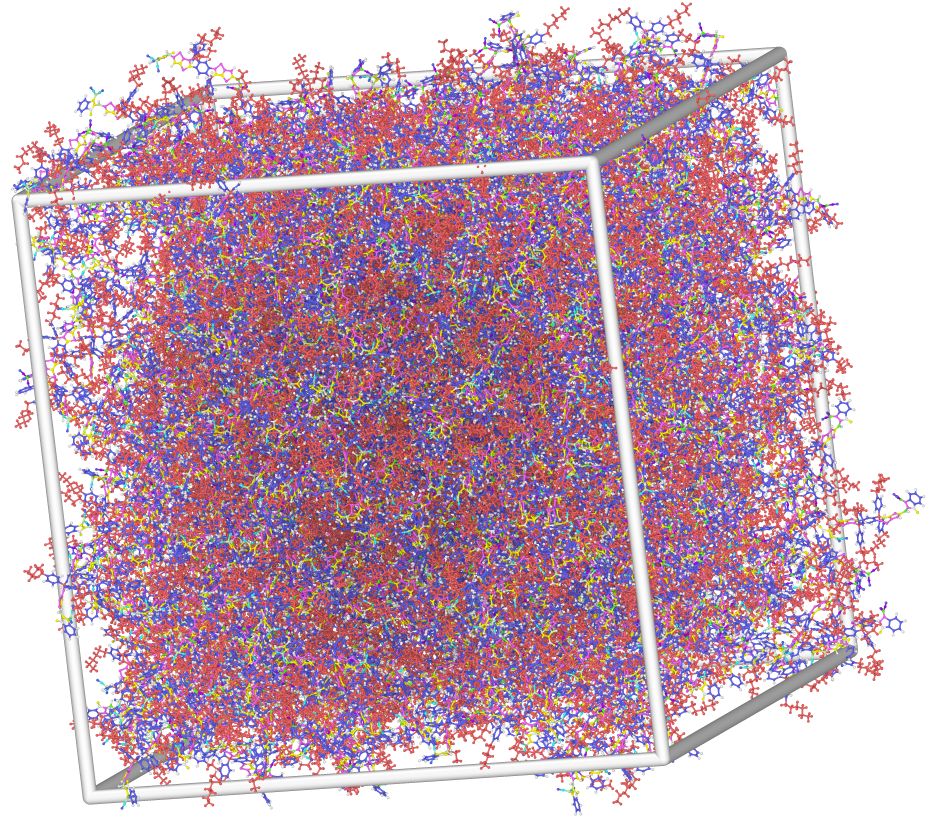
\includegraphics[width=\textwidth]{figures/ITIC-blackedout-unwrapped-allatom.png}
\end{subfigure}%
\begin{subfigure}{.5\textwidth}
    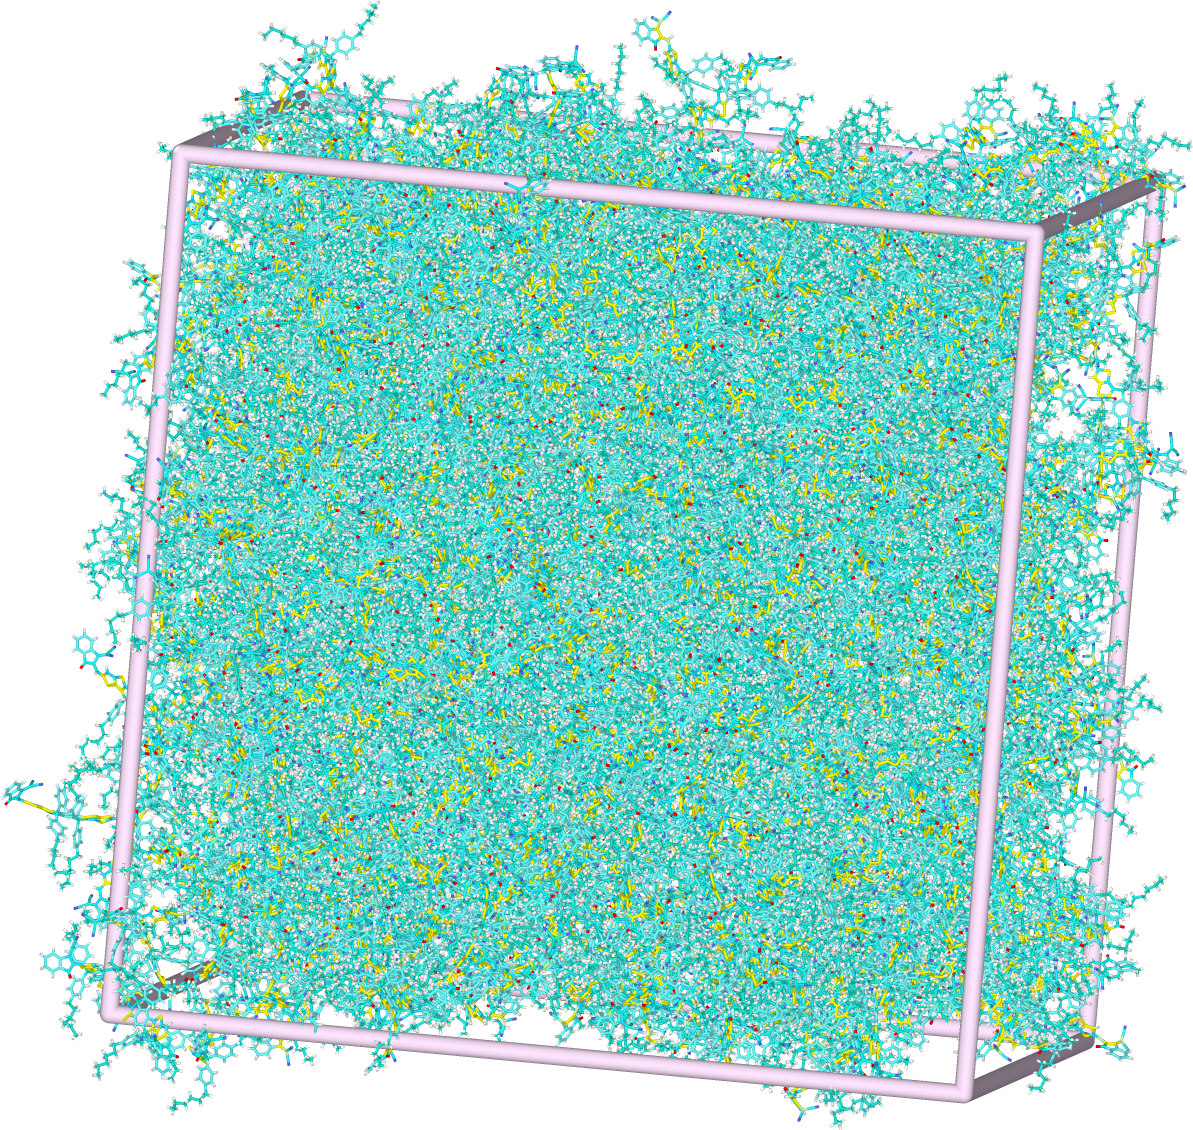
\includegraphics[width=\textwidth]{figures/ITIC-unwrapped.png}
\end{subfigure}
    \caption{$1000$ molecule \glsxtrshort{itic} morphology. Colored atoms were included in the
    \gls{qcc}s for the backbone chromophore simutlation (LEFT) and whole molecule chromophore simulations
    (RIGHT).}
\label{ITIC}
\end{figure}

A single molecule of \glsxtrshort{itic} has 186 atoms, with the backbone consisting of 70 atoms. We deployed two different
approaches to the delineation of chromophores within the \glsxtrshort{itic} morphology. 
We first take the backbone to be the chromophores. In another simulation, we
take the whole molecule to be a chromophore. 

Including the whole molecule necessarily requires more heavy lifting from \texttt{pySCF} but is trivially easy from an indexing perspective.
Similar to the results of the $d_{cut}$ investigation, 
this implementation of \texttt{pySCF}, combined with clever pickling of system objects at various stages
of the workflow, suggest that the laborious delineation of chromophores can be
largely circumvented in macromolecular systems like \gls{itic}.
We found that, while the 70 atom chromophores took $1.2s$ 
per dimer while, the whole molecule dimer calculations with 186 atoms per
chromophore took on average $3.3s$. This is a substantial increase across a
hundred thousand pair calculation. However, as we have seen in
\autoref{morphct}, organizing a workflow that ensures that this step only be
performed once minimizes the computational blow.

We found comparable mobilities of $(1.019 \pm 0.001)\cdot 10^{-3}$ for the backbone chromophores and 
$(1.275 \pm 0.001)\cdot 10^{-3}$ for the whole molecule. This increase in
mobility comports with the reality, as including the side chains adds some
electron density off the axis of the backbone which could facilitated hopping
pathways unexplored by the backbone only simulations. While the contribution
from the electron density along the side chains is minimal when discussing
mobility values that vary orders of magnitude, the contribution is not zero.


As discussed in the sensitivity analysis, our mobility calculations are relatively sensitive to the choice of
reorganization energy. For \glsxtrshort{itic}, $\lambda_{internal}$ has been well investigated and is widely reported as
$~0.15eV$ \cite{Han2019}. The external reorganization is harder to estimate. We take $\lambda_{total}=0.3eV$ as we did for
\glsxtrshort{p3ht}. With the fused
backbone resulting in a higher internal contribution and the lack of long range order resulting in a lower
external contribution. 

The reported experimental electron mobility of \glsxtrshort{itic} varies depending on how it was processed and how it was measured. 
Time-of-flight electron mobilities on the order of $10^{-4}$ \cite{Mica2018} and field effect mobilities on the order of
$10^{-2}$ \cite{Park2018} have been reported. Another computational study, that also used Marcus hopping and
\gls{kmc}, found an electron mobility of $7\cdot10^{-4}$~\cite{Han2017b} in a pure \gls{itic} crystal.


%%% Local Variables: 
%%% mode: latex
%%% TeX-master: "BSUmain"
%%% End: 
